\documentclass[a4paper, 12pt]{article}

% packages
\usepackage{amssymb}
\usepackage[fleqn]{mathtools}
\usepackage{tikz}
\usepackage{enumerate}
\usepackage{bussproofs}
\usepackage{xcolor}
\usepackage[margin=1.3cm]{geometry}
\usepackage{logicproof}
\usepackage{diagbox}
\usepackage{listings}
\usepackage{graphicx}
\usepackage{lstautogobble}
\usepackage{hyperref}
\usepackage{multirow}
\usepackage{tipa}
\usepackage{pgfplots}
\usepackage{adjustbox}
\usepackage[nocomma]{optidef}

% tikz libraries
\usetikzlibrary{
    decorations.pathreplacing,
    arrows,
    shapes,
    shapes.gates.logic.US,
    circuits.logic.US,
    calc,
    automata,
    positioning,
    intersections
}

\pgfplotsset{compat=1.16}
\usepgfplotslibrary{fillbetween}
\pgfmathdeclarefunction{gauss}{2}{%
  \pgfmathparse{1/(#2*sqrt(2*pi))*exp(-((x-#1)^2)/(2*#2^2))}%
}

\allowdisplaybreaks % allow environments to break
\setlength\parindent{0pt} % no indent

% shorthand for verbatim
% this clashes with logicproof, so maybe fix this at some point?
% \catcode`~=\active
% \def~#1~{\texttt{#1}}

% code listing
\lstdefinestyle{main}{
    numberstyle=\tiny,
    breaklines=true,
    showspaces=false,
    showstringspaces=false,
    tabsize=2,
    numbers=left,
    basicstyle=\ttfamily,
    columns=fixed,
    fontadjust=true,
    basewidth=0.5em,
    autogobble,
    xleftmargin=3.0ex,
    mathescape=true
}
\newcommand{\dollar}{\mbox{\textdollar}} %
\lstset{style=main}

% augmented matrix
\makeatletter
\renewcommand*\env@matrix[1][*\c@MaxMatrixCols c]{%
\hskip -\arraycolsep
\let\@ifnextchar\new@ifnextchar
\array{#1}}
\makeatother

% ceiling / floor
\DeclarePairedDelimiter{\ceil}{\lceil}{\rceil}
\DeclarePairedDelimiter{\floor}{\lfloor}{\rfloor}

% custom commands
\newcommand{\indefint}[2]{\int #1 \, \mathrm{d}#2}
\newcommand{\defint}[4]{\int_{#1}^{#2} #3 \, \mathrm{d}#4}
\newcommand{\pdif}[2]{\frac{\partial #1}{\partial #2}}
\newcommand{\dif}[2]{\frac{\mathrm{d}#1}{\mathrm{d}#2}}
\newcommand{\limit}[2]{\raisebox{0.5ex}{\scalebox{0.8}{$\displaystyle{\lim_{#1 \to #2}}$}}}
\newcommand{\limitsup}[2]{\raisebox{0.5ex}{\scalebox{0.8}{$\displaystyle{\limsup_{#1 \to #2}}$}}}
\newcommand{\summation}[2]{\sum\limits_{#1}^{#2}}
\newcommand{\product}[2]{\prod\limits_{#1}^{#2}}
\newcommand{\intbracket}[3]{\left[#3\right]_{#1}^{#2}}
\newcommand{\laplace}{\mathcal{L}}
\newcommand{\fourier}{\mathcal{F}}
\newcommand{\mat}[1]{\boldsymbol{#1}}
\renewcommand{\vec}[1]{\boldsymbol{#1}}
\newcommand{\rowt}[1]{\begin{bmatrix}
    #1
\end{bmatrix}^\top}
\DeclareMathOperator*{\argmax}{argmax}
\DeclareMathOperator*{\argmin}{argmin}

\newcommand{\lto}[0]{\leadsto\ }

\newcommand{\ulsmash}[1]{\underline{\smash{#1}}}

\newcommand{\powerset}[0]{\wp}
\renewcommand{\emptyset}[0]{\varnothing}

\makeatletter
\newsavebox{\@brx}
\newcommand{\llangle}[1][]{\savebox{\@brx}{\(\m@th{#1\langle}\)}%
  \mathopen{\copy\@brx\kern-0.5\wd\@brx\usebox{\@brx}}}
\newcommand{\rrangle}[1][]{\savebox{\@brx}{\(\m@th{#1\rangle}\)}%
  \mathclose{\copy\@brx\kern-0.5\wd\@brx\usebox{\@brx}}}
\makeatother
\newcommand{\lla}{\llangle}
\newcommand{\rra}{\rrangle}
\newcommand{\la}{\langle}
\newcommand{\ra}{\rangle}
\newcommand{\crnr}[1]{\text{\textopencorner} #1 \text{\textcorner}}
\newcommand{\bnfsep}[0]{\ |\ }
\newcommand{\concsep}[0]{\ ||\ }

\newcommand{\axiom}[1]{\AxiomC{#1}}
\newcommand{\unary}[1]{\UnaryInfC{#1}}
\newcommand{\binary}[1]{\BinaryInfC{#1}}
\newcommand{\trinary}[1]{\TrinaryInfC{#1}}
\newcommand{\quaternary}[1]{\QuaternaryInfC{#1}}
\newcommand{\quinary}[1]{\QuinaryInfC{#1}}
\newcommand{\dproof}[0]{\DisplayProof}
\newcommand{\llabel}[1]{\LeftLabel{\scriptsize #1}}
\newcommand{\rlabel}[1]{\RightLabel{\scriptsize #1}}

\newcommand{\ttbs}{\char`\\}
\newcommand{\lrbt}[0]{\ \bullet\ }

% colours
\newcommand{\violet}[1]{\textcolor{violet}{#1}}
\newcommand{\blue}[1]{\textcolor{blue}{#1}}
\newcommand{\red}[1]{\textcolor{red}{#1}}
\newcommand{\teal}[1]{\textcolor{teal}{#1}}

% reasoning proofs
\usepackage{ltablex}
\usepackage{environ}
\keepXColumns
\NewEnviron{reasoning}{
    \begin{tabularx}{\textwidth}{rlX}
        \BODY
    \end{tabularx}
}
\newcommand{\proofline}[3]{$(#1)$ & $#2$ & \hfill #3 \smallskip \\}
\newcommand{\proofarbitrary}[1]{& take arbitrary $#1$ \smallskip \\}
\newcommand{\prooftext}[1]{\multicolumn{3}{l}{#1} \smallskip \\}
\newcommand{\proofmath}[3]{$#1$ & = $#2$ & \hfill #3 \smallskip \\}
\newcommand{\prooftherefore}[1]{& $\therefore #1$ \smallskip \\}
\newcommand{\proofbc}[0]{\prooftext{\textbf{Base Case}}}
\newcommand{\proofis}[0]{\prooftext{\textbf{Inductive Step}}}

% ER diagrams
\newcommand{\nattribute}[4]{
    \node[draw, state, inner sep=0cm, minimum size=0.2cm, label=#3:{#4}] (#1) at (#2) {};
}
\newcommand{\mattribute}[4]{
    \node[draw, state, accepting, inner sep=0cm, minimum size=0.2cm, label=#3:{#4}] (#1) at (#2) {};
}
\newcommand{\dattribute}[4]{
    \node[draw, state, dashed, inner sep=0cm, minimum size=0.2cm, label=#3:{#4}] (#1) at (#2) {};
}
\newcommand{\entity}[3]{
    \node[] (#1-c) at (#2) {#3};
    \node[inner sep=0cm] (#1-l) at ($(#1-c) + (-1, 0)$) {};
    \node[inner sep=0cm] (#1-r) at ($(#1-c) + (1, 0)$) {};
    \node[inner sep=0cm] (#1-u) at ($(#1-c) + (0, 0.5)$) {};
    \node[inner sep=0cm] (#1-d) at ($(#1-c) + (0, -0.5)$) {};
    \draw
    ($(#1-c) + (-1, 0.5)$) -- ($(#1-c) + (1, 0.5)$) -- ($(#1-c) + (1, -0.5)$) -- ($(#1-c) + (-1, -0.5)$) -- cycle;
}
\newcommand{\relationship}[3]{
    \node[] (#1-c) at (#2) {#3};
    \node[inner sep=0cm] (#1-l) at ($(#1-c) + (-1, 0)$) {};
    \node[inner sep=0cm] (#1-r) at ($(#1-c) + (1, 0)$) {};
    \node[inner sep=0cm] (#1-u) at ($(#1-c) + (0, 1)$) {};
    \node[inner sep=0cm] (#1-d) at ($(#1-c) + (0, -1)$) {};
    \draw
    ($(#1-c) + (-1, 0)$) -- ($(#1-c) + (0, 1)$) -- ($(#1-c) + (1, 0)$) -- ($(#1-c) + (0, -1)$) -- cycle;
}

% AVL Trees
\newcommand{\avltri}[4]{
    \draw ($(#1)$) -- ($(#1) + #4*(0.5, -1)$) -- ($(#1) + #4*(-0.5, -1)$) -- cycle;
    \node at ($(#1) + #4*(0, -1) + (0, 0.5)$) {#3};
    \node at ($(#1) + #4*(0, -1) + (0, -0.5)$) {#2};
}

% RB Trees
\tikzset{rbtr/.style={inner sep=2pt, circle, draw=black, fill=red}}
\tikzset{rbtb/.style={inner sep=2pt, circle, draw=black, fill=black}}

% Samples
\tikzset{spos/.style={inner sep=2pt, circle, draw=black, fill=blue!20}}
\tikzset{sneg/.style={inner sep=2pt, circle, draw=black, fill=red!20}}

% Joins
\newcommand\ljoin{\stackrel{\mathclap{\normalfont\mbox{\tiny L}}}{\bowtie}}
\newcommand\rjoin{\stackrel{\mathclap{\normalfont\mbox{\tiny R}}}{\bowtie}}
\newcommand\ojoin{\stackrel{\mathclap{\normalfont\mbox{\tiny O}}}{\bowtie}}

\setcounter{MaxMatrixCols}{100}

% actual document
\begin{document}
    {\sc Computing $3^\text{rd}$ Year Notes} \hfill \texttt{https://github.com/lin-e/imperial-revision}
    \rule{\textwidth}{0.1pt}
    \section*{CO343 - Operations Research \hfill (60016)}
        \subsection*{Lecture 1}
            Operations research is the science of taking decisions, it's a branch of applied mathematics where we attempt to model problems where need to make a decision.
            The decisions aren't arbitrary, and we want to attempt to score each decision based on some metric (such as time, cost, etc.), to find the optimal solution.
            \medskip

            The course focuses on formulating a mathematical model to represent the problem, and then developing a computer-based procedure for deriving solutions to the problem from the model.
            Assume our goal was the following;
            $$\min_{\vec{x}} z = f(\vec{x}) \hspace{50pt} \text{subject to } \vec{x} \in \mathcal{X}$$
            \begin{itemize}
                \itemsep0em
                \item \textbf{decision variables} \hfill $\vec{x} \in \mathbb{R}^n$
                \item \textbf{objective function} \hfill $f : \mathbb{R}^n \to \mathbb{R}$
                \item \textbf{feasible set} (set of admissible decisions) \hfill $\mathcal{X} \subseteq \mathbb{R}^n$
                \item \textbf{optimal solution} (any vector that minimises $f$) \hfill $\vec{x^*}$
                \item \textbf{optimal value} \hfill $z^* = f(\vec{x^*})$
            \end{itemize}
            \subsubsection*{Linear Programming}
                A linear program optimises a \textbf{linear objective function}, where a feasible set is described by linear equality / inequality constraints.
                Compared to non-linear problems, where a \textbf{local} maximum may vary (and therefore be sub-optimal) depending on the starting search position, this isn't a concern for linear problems.
                \medskip

                We can say the polygon representing a two dimensional feasible set is convex if the points on the line joining two points in the feasible set are also in the polygon.
                If this region is convex and linear, it can be proven that a local optimum is also a global optimum.
                For example, take $x$ and $x^\prime$;
                \begin{center}
                    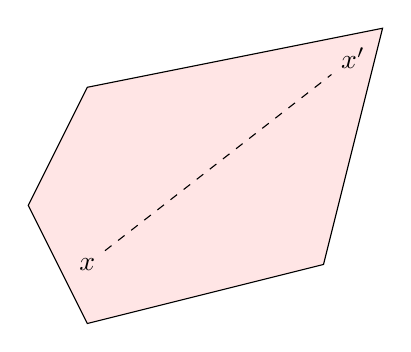
\begin{tikzpicture}[x=0.75cm, y=0.75cm]
                        \draw[fill=red!10]
                        (0, 0) -- (5, 1) -- (4, -3) -- (0, -4) -- (-1, -2) -- cycle;

                        \node (x) at (0, -3) {$x$};
                        \node (xp) at (4.5, 0.5) {$x^\prime$};

                        \draw (x) edge[dashed] (xp);
                    \end{tikzpicture}
                \end{center}
            \subsubsection*{Linear Programming Example}
                A manufacturer produces $A$ (acid) and $C$ (caustic) and wants to decide a production plan.
                The ingredients for $A$ and $C$ are $X$ (a sulphate) and $Y$ (sodium).
                \begin{itemize}
                    \itemsep0em
                    \item each ton of $A$ requires 2 tons of $X$ and 1 ton of $Y$
                    \item each ton of $C$ requires 1 ton of $X$ and 3 tons of $Y$
                    \item supply of $X$ is limited to 11 tons per week
                    \item supply of $Y$ is limited to 18 tons per week
                    \item $A$ sells for £1000 per ton
                    \item $C$ sells for £1000 per ton
                    \item a maximum of 4 tons of $A$ can be sold per week
                \end{itemize}
                Our goal is to maximise weekly value of sales of $A$ and $C$.
                To determine how much $A$ and $C$ to produce, we need to formulate a \textbf{mathematical programming model};
                \begin{itemize}
                    \itemsep0em
                    \item \textbf{decision variables}
                        \begin{itemize}
                            \itemsep0em
                            \item weekly production of $A$ (tons) \hfill $x_1$
                            \item weekly production of $B$ (tons) \hfill $x_2$
                        \end{itemize}
                    \item \textbf{objective function} (weekly profit in £1000s) \hfill $z = f(x_1, x_2)$
                    \item \textbf{feasible set} \hfill $\vec{x} = (x_1, x_2) \in \mathcal{X}$
                \end{itemize}
                A \textbf{production plan} is representable as $\vec{x} = (x_1, x_2)$.
                The objective function can be written as $z = x_1 + x_2$.
                Another constraint is that \violet{$x_1 \geq 0$} and \violet{$x_2 \geq 0$}; we cannot produce a negative amount of a product.
                $x_1$ tons of $A$ and $x_2$ tons of $C$ requires $2x_1 + x_2$ tons of $X$, and we know that is limited to 11 tons per week; therefore we have the constraint \blue{$2x_1 + x_2 \leq 11$}.
                Similarly, we also have the limitation of \red{$x_1 + 3x_2 \leq 18$}, because of the limitations of $Y$.
                Finally, we have another restriction that we cannot sell more than 4 tons of $A$, therefore \teal{$x_1 \leq 4$}.
                \medskip

                To get the overall feasible set, we intersect the feasible set of all the constraints to get the following;
                \begin{center}
                    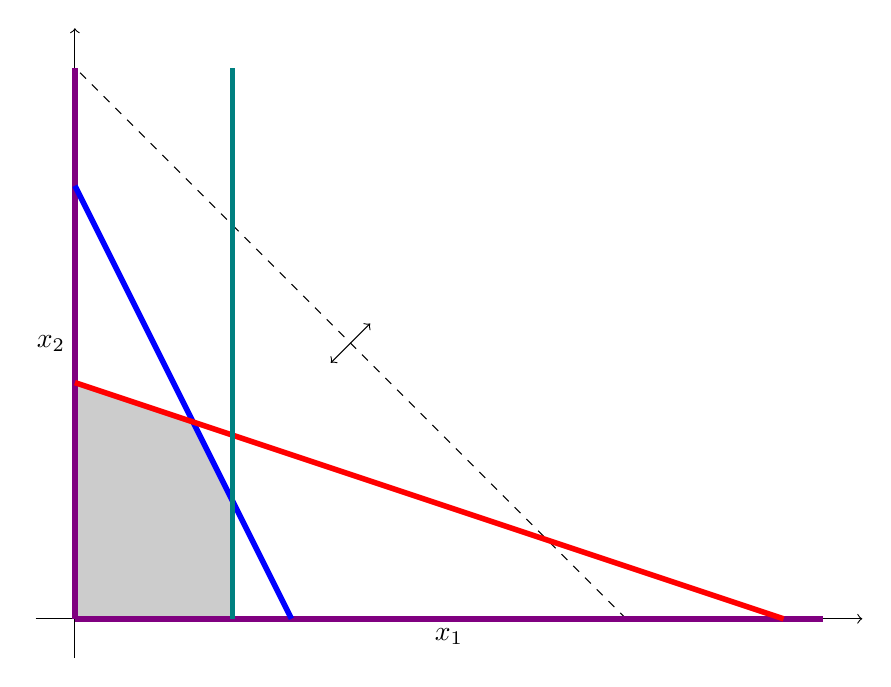
\begin{tikzpicture}[x=0.5cm, y=0.5cm]
                        \draw
                        (0, -1) edge[->, left] node{$x_2$} (0, 15)
                        (-1, 0) edge[->, below] node{$x_1$} (20, 0);

                        \draw
                        (14, 0) edge[dashed] (0, 14)
                        (6.5, 6.5) edge[<->] (7.5, 7.5);

                        \draw[fill=black!20] (0, 0) -- (0, 6) -- (3, 5) -- (4, 3) -- (4, 0) -- cycle;

                        \draw
                        (0, 0) edge[violet, line width=2pt] (0, 14)
                        (0, 0) edge[violet, line width=2pt] (19, 0)
                        (0, 11) edge[blue, line width=2pt] (5.5, 0)
                        (0, 6) edge[red, line width=2pt] (18, 0)
                        (4, 0) edge[teal, line width=2pt] (4, 14);
                    \end{tikzpicture}
                \end{center}
                Each of the following vertices is the intersection of constraints, which can be obtained by solving the linear equation of each line;
                \begin{align*}
                    O & = (0, 0) \\
                    P & = (0, 6) \\
                    Q & = (3, 5) \\
                    R & = (4, 3) \\
                    S & = (4, 0)
                \end{align*}
                By moving the objective function (the dashed line), in the direction of the arrows, we can see that the $z$ value increases further away from the origin, and therefore the graphical result that results in the highest value is $Q$.
                Typically the optimal solution lies on a vertex, however in some cases, there can be multiple solutions (an edge when the objective function is parallel to the constraint, or all the points in the feasible set in the case of a constant objective function).
                \medskip

                The simplest algorithm is to enumerate all the vertices (intersections) of the feasible set, however this can have exponential complexity in the worst case and the number of vertices grow quite quickly in higher dimensions.
                The \textbf{Simplex Algorithm} finds an optimal vertex, often inspecting a \textbf{small subset} of the total.
                \medskip

                We can vary this example, for example if we wanted to minimise $z = 3x_1 - x_2$ over the feasible set, we can examine the objective function at each of the vertices;
                \begin{center}
                    \begin{tabular}{c|c|c|c|c}
                        $O = (0, 0)$ & $P = (0, 6)$ & $Q = (3, 5)$ & $R = (4, 3)$ & $S = (4, 0)$ \\
                        \hline
                        0 & -6 & 4 & 9 & 12
                    \end{tabular}
                \end{center}
                This therefore gives us $P = (x_1, x_2) = (0, 6)$ as the optimal.
                \medskip

                On the other hand, if we were to maximise $z = 2x_1 + x_2$, any point on the line segment $QR$ would be optimal; this tells us that points other than the vertices can be optimal, but there is at least one optimal vertex.
                \medskip

                Additionally, if we were to set a production goal of 7 tons of $A$, we'd have an empty feasible set, since $x_1 \geq 7$ would cause an empty set with $x_1 \leq 4$.
                In this case, the LP is \textbf{infeasible}.
                Similarly, if the constraints on $X$ and $Y$ were removed, the objective function could grow to $+\infty$, hence the LP is \textbf{unbounded}.
        \subsection*{Lecture 2}
            \subsubsection*{Standard Form}
                In order to use a computer to solve an LP problem, we need to define a \textbf{standard form};
                \begin{itemize}
                    \itemsep0em
                    \item the goal is to \textbf{minimise} a \textbf{linear} objective function
                    \item all constraints are linear equality constraints
                    \item all constraint right hand sides are non-negative
                    \item all decision variables are non-negative
                \end{itemize}
                A linear problem in standard form is as follows;
                $$\begin{matrix}
                    \text{minimise} & z = c_1 x_1 & + & c_2 x_2 & + & \cdots & c_n x_n \\ \\
                    \text{subject to} & a_{1, 1} x_1 & + & a_{1, 2} x_2 & + & \cdots & a_{1, n} x_n & = & b_1 \\
                    & a_{2, 1} x_1 & + & a_{2, 2} x_2 & + & \cdots & a_{2, n} x_n & = & b_2 \\
                    & \vdots & & \vdots & & & \vdots & & \vdots \\
                    & a_{m, 1} x_1 & + & a_{m, 2} x_2 & + & \cdots & a_{m, n} x_n & = & b_m
                \end{matrix}$$
                This has the constraints that all decision variables $\forall i \in [1, n]\ x_i \geq 0$ and $\forall i \in [1, m]\ b_i \geq 0$.
                The \textbf{input parameters} $b_i$, $c_j$, and $a_{i, j}$ are fixed real constants.
                Clearly, this can be written more compactly as the following;
                \begin{align*}
                    \mat{A} & = \begin{bmatrix}
                        a_{1, 1} & a_{1, 2} & \cdots & a_{1, n} \\
                        a_{2, 1} & a_{2, 2} & \cdots & a_{2, n} \\
                        \vdots & \vdots & \ddots & \vdots \\
                        a_{m ,1} & a_{m, 2} & \cdots & a_{m, n}
                    \end{bmatrix} \\
                    \vec{b} & = \begin{bmatrix}
                        b_1 \\ b_2 \\ \vdots \\ b_m
                    \end{bmatrix} \\
                    \vec{x} & = \begin{bmatrix}
                        x_1 \\ x_2 \\ \vdots \\ x_n
                    \end{bmatrix} \\
                    \vec{c} & = \begin{bmatrix}
                        c_1 \\ c_2 \\ \vdots \\ c_n
                    \end{bmatrix}
                \end{align*}
                Therefore, the equation can be written as;
                $$\text{minimise } \vec{z} = \vec{c}^\top \vec{x} \text{ subject to } \mat{A}\vec{x} = \vec{b}$$
                Note that $\vec{x} \geq 0$ and $\vec{b} \geq 0$, which means that it holds \textbf{component-wise} (such that $\forall x_i \in \vec{x}\ x_i \geq 0$).
            \subsubsection*{Standardising}
                This follows the example in tutorial 1.
                \medskip

                Our goal is to maximise $y = 2x_1 + x_2$, (s.t.) subject to;
                \begin{itemize}
                    \itemsep0em
                    \item $x_1 - 4x_2 \leq 1$
                    \item $-x_1 - 5x_2 \leq -3$
                    \item $x_1, x_2 \geq 0$
                \end{itemize}
                We can do the following conversion steps to get the equations into the standard form.
                To reformulate inequalities as equalities, we introduced the \textbf{slack variables} $s_1$ and $s_2$.
                All that is left to do is to convert the maximisation into a minimisation, which can be done by negating the objective function.
                \begin{align*}
                    x_1 - 4x_2 & \leq 1 & \Rightarrow \\
                    x_1 - 4x_2 + \violet{s_1} & = 1 \\
                    -x_1 - 5x_2 & \leq 3 & \Rightarrow \\
                    x_1 + 5x_2 & \geq -3 & \Rightarrow \\
                    x_1 + 5x_2 - \blue{s_2} & = -3 \\
                    x_1, x_2, \violet{s_1}, \blue{s_2} & \geq 0 \\
                    \text{(maximise) } y & = 2x_1 + x_2 & \Rightarrow \\
                    \text{(minimise) } z & = -2x_1 - x_2
                \end{align*}
                Therefore, we can therefore say a minimisation of $\vec{z} = \vec{c}^\top\vec{x}$ subject to $\mat{A}\vec{x} \leq \vec{b}$ and $\vec{x} \geq 0$ is equivalent to the same minimisation subject to $\mat{A}\vec{x} + \vec{s} = \vec{b}$ and $\vec{x}, \vec{s} \geq 0$.
                The slack variables take the value of the difference $\vec{b} - \mat{A}\vec{x}$.
                Similarly, \textbf{excess variables} are the same, but instead of being added to the left hand side of the inequality, they are subtracted, and therefore take the value of the difference $\mat{A}\vec{x} - \vec{b}$.
                Additionally, a change of sign for the right hand side is trivial, as it can be done by multiplying the entire inequality by $-1$.
            \subsubsection*{Free Variables}
                Suppose the constraint $x_j \geq 0$ does not exist, such that it can be positive or negative.
                We can do this by substituting $x_j = x_j^+ - x_j^-$.
                The LP now has the following $n + 1$ variables;
                $$x_1, \dots, x_{j - 1}, x_j^+, x_j^-, x_{j + 1}, \dots, x_n$$
                Another approach to introduce free variables is to use substitution.
                Any \textbf{equality constraint} involving $x_j$ can be used to eliminate $x_j$, as for $x_1$ in the following conditions (with the substitution of $x_1 = 5 - 3x_2 - x_3$);
                \begin{align*}
                    \text{(minimise) } z & = x_1 + 3x_2 + 4x_3 \\
                    x_1 + 2x_2 + x_3 & = 5 \\
                    2x_1 + 3x_2 + x_3 & = 6 & \Rightarrow \\ \\
                    \violet{\text{(minimise) } z} &\ \violet{= x_2 + 3x_3 + 5} \\
                    \violet{x_2 + x_3} &\ \violet{= 4}
                \end{align*}
            \subsubsection*{Tutorial}
                \begin{enumerate}[1.]
                    \itemsep0em
                    \setcounter{enumi}{1}
                    \item
                        A company produces laptops at two factories, $A$ and $B$.
                        In factory $A$, $s_A$ laptops are produced a year, and $s_B$ laptops are produced a year in factory $B$.
                        The three stores, 1, 2, and 3, sell $d_1$, $d_2$, and $d_3$ a year.
                        The cost of shipping a laptop from the factory $i \in \{A, B\}$ to store $j \in \{1, 2, 3,\}$ is $c_{i, j}$.
                        Assume that the demand of all stores can be satisfied, such that $s_A + s_B \geq d_1 + d_2 + d_3$.
                        \begin{enumerate}[1.]
                            \itemsep0em
                            \item How should the laptops be shipped from the two factories to minimise shipping costs, assuming the following;
                                \begin{align*}
                                    \begin{bmatrix}
                                        s_A \\ s_B
                                    \end{bmatrix} & = \begin{bmatrix}
                                        3 \\ 3
                                    \end{bmatrix} \\
                                    \begin{bmatrix}
                                        d_1 \\ d_2 \\ d_3
                                    \end{bmatrix} & = \begin{bmatrix}
                                        2 \\ 2 \\ 2
                                    \end{bmatrix} \\
                                    (c_{i, j}) & = \begin{bmatrix}
                                        1 & 2 & 1 \\
                                        2 & 1 & 2
                                    \end{bmatrix} & \text{(first row corresponds to store $A$)}
                                \end{align*}
                            \item Formulate the optimisation model corresponding to the previous question, using the general parameters;
                                \medskip

                                Note that we will denote the number of laptops from each factory $i \in \{A, B\}$ to store $j \in \{1, 2, 3\}$ as $x_{i, j}$.
                                We therefore want to minimise the following;
                                $$z = \summation{i}{} \summation{j}{} c_{i, j}x_{i, j}$$
                                Under the following conditions;
                                \begin{align*}
                                    x_{A, j} + x_{B, j} & = d_j & \forall j \in \{1, 2, 3\} \\
                                    x_{i, 1} + x_{i, 2} + x_{i, 3} & \leq s_i & \forall i \in \{A, B\} \\
                                    x_{i, j} & \geq 0 & \forall i, \forall j
                                \end{align*}
                                It's important to note that satisfying demand is to use equality, as we can reduce the amount of computation we need to do.
                        \end{enumerate}
                \end{enumerate}
        \subsection*{Lecture 3}
            We now only focus on LPs in \textbf{standard form};
            minimise $z = \vec{c}^\top\vec{x}$, subject to $\mat{A}\vec{x} = \vec{b}$ and $\vec{x} \geq 0$, where $\mat{A} \in \mathbb{R}^{m \times n}, \vec{b} \in \mathbb{R}^m \geq 0, c \in \mathbb{R}^n$.
            We also assume that (the number of variables) $n \geq m$ (the number of equations), otherwise the system $\mat{A}\vec{x} = \vec{b}$ is overdetermined.
            Similarly, we also assume that the rows of $\mat{A}$ are linearly independent, otherwise constraints are redundant or consistent.
            Therefore, we can say $\text{rk}(\mat{A}) = m$.
            If there is linear dependence, we have either;
            \begin{itemize}
                \itemsep0em
                \item \textbf{contradictory constraints} (no solution)
                    \begin{align*}
                        x_1 + x_2 & = 1 \\
                        x_1 + x_2 & = 2
                    \end{align*}
                \item \textbf{redundant constraints}
                    \begin{align*}
                        x_1 + x_2 & = 1 \\
                        2x_1 + 2x_2 & = 2
                    \end{align*}
            \end{itemize}
            For now, we focus only on the system of linear equations in $\mathcal{LP}$;
            $$\mat{A}\vec{x} = \vec{b}$$
            Let $\mat{A} = [\vec{a_1}, \dots, \vec{a_n}]$ where $a_i \in \mathbb{R}^m$ is the $i^\text{th}$ column vector of $\mat{A}$.
            We want to select a subset of $m$ columns $\vec{a_i}$ that are linearly independent - which will always be possible since $n \geq m = \text{rk}(\mat{A})$.
            This gives us a square matrix for us to solve.
            The \textbf{index set} $I$ consists of the indices for those $m$ columns, hence $I \subseteq \{1, \dots, n\}$.
            We define the matrix $\mat{B} = B(I) \in \mathbb{R}^{m \times m}$ consisting of the columns $\{\vec{a_i}\}_{i \in I}$ as the \textbf{basis} corresponding to the index set $I$.
            \medskip

            We define a solution $\vec{x}$ to $\mat{A}\vec{x} = \vec{b}$ with $\forall i \notin I\ (x_i = 0)$ as a \textbf{basic solution (BS)} to $\mat{A}\vec{x} = \vec{b}$ with respect to the index set $I$.
            Similarly, we define a solution $\vec{x}$ satisfying both $\mat{A}\vec{x} = \vec{b}$ and $\vec{x} \geq 0$ as a \textbf{feasible solution (FS)}.
            A feasible solution, which is also basic, is a \textbf{basic feasible solution (BFS)}.
            \medskip

            Assume, for the example $I = \{1, \dots, m\}$.
            $$\begin{matrix}
                a_{1, 1}x_1 & + & \dots & + & a_{1, m}x_m & + & a_{1, m + 1}x_{m + 1} & + & \dots & + & a_{1, n}x_n & = & b_1 \\
                a_{2, 1}x_1 & + & \dots & + & a_{2, m}x_m & + & a_{2, m + 1}x_{m + 1} & + & \dots & + & a_{2, n}x_n & = & b_2 \\
                \vdots & & & & \vdots & & \vdots & & & & \vdots & & \vdots \\
                a_{m, 1}x_1 & + & \dots & + & a_{m, m}x_m & + & a_{m, m + 1}x_{m + 1} & + & \dots & + & a_{m, n}x_n & = & b_m
            \end{matrix}$$
            This is then equivalent to $\mat{B}\vec{x_B} = \vec{b}$;
            $$\begin{matrix}
                a_{1, 1}x_1 & + & \dots & + & a_{1, m}x_m & + & a_{1, m + 1}0 & + & \dots & + & a_{1, n}0 & = & b_1 \\
                a_{2, 1}x_1 & + & \dots & + & a_{2, m}x_m & + & a_{2, m + 1}0 & + & \dots & + & a_{2, n}0 & = & b_2 \\
                \vdots & & & & \vdots & & \vdots & & & & \vdots & & \vdots \\
                a_{m, 1}x_1 & + & \dots & + & a_{m, m}x_m & + & a_{m, m + 1}0 & + & \dots & + & a_{m, n}0 & = & b_m
            \end{matrix}$$
            By removing the 0 terms, we can simplify it to the following;
            $$\begin{matrix}
                a_{1, 1}x_1 & + & \dots & + & a_{1, m}x_m & = & b_1 \\
                a_{2, 1}x_1 & + & \dots & + & a_{2, m}x_m & = & b_2 \\
                \vdots & & & & \vdots & & \vdots \\
                a_{m, 1}x_1 & + & \dots & + & a_{m, m}x_m & = & b_m
            \end{matrix}$$
            We can observe that the \textbf{basic solution} corresponding to $I$ is unique, since the vectors $\{\vec{a_i}\}_{i \in I}$ are linearly independent, the basis $\mat{B}$ is invertible, and has the following unique solution;
            $$\vec{x_B} = \mat{B}^{-1}\vec{b} \in \mathbb{R}^m$$
            Therefore, we can define the vector $\vec{x}$ as;
            $$x_i = \begin{cases}
                \vec{x_B}_i & i \in I \\
                0 & i \notin I
            \end{cases}$$
            This $\vec{x}$ is the \textbf{unique basic solution} to $\mat{A}\vec{x} = \vec{b}$ with respect to $I$.
            However - this doesn't mean it's feasible, as we could end up with negative values.
            The geometric intuition that the corners of the feasible set correspond are LP come back into play, when we consider that the corners of the feasible set correspond to \textbf{basic feasible solutions}.
            \medskip

            Consider the example from the first lecture (note that each line in the previously drawn graph denotes when a variable in the standard form is zero);
            \begin{align*}
                y & = x_1 + x_2 & \text{objective function} \\
                2x_1 + x_2 & \leq 11 & \text{constraint on availability of $X$} \\
                x_1 + 3x_2 & \leq 18 & \text{constraint on availability of $Y$} \\
                x_1 & \leq 4 & \text{constraint on demand of $A$} \\
                x_1, x_2 & \geq 0 & \text{non-negativity constraints}
                \intertext{In standard form:}
                n & = 5 & \text{number of variables} \\
                m & = 3 & \text{number of constraints} \\
                z & = -x_1 - x_2 & \text{objective function} \\
                2x_1 + x_2 + x_3 & = 11 \\
                x_1 + 3x_2 + x_4 & = 18 \\
                x_1 + x_5 & = 4 \\
                x_1, x_2, x_3, x_4, x_5 & \geq 0
            \end{align*}
            \begin{center}
                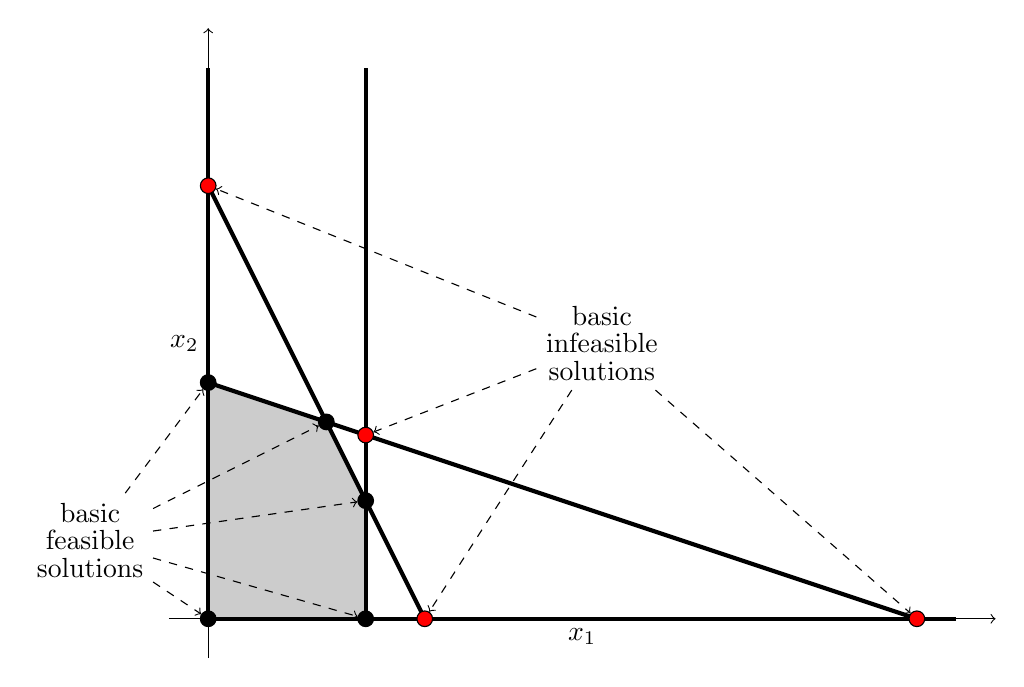
\begin{tikzpicture}[x=0.5cm, y=0.5cm]
                    \draw
                    (0, -1) edge[->, left] node{$x_2$} (0, 15)
                    (-1, 0) edge[->, below] node{$x_1$} (20, 0);

                    \draw[fill=black!20] (0, 0) -- (0, 6) -- (3, 5) -- (4, 3) -- (4, 0) -- cycle;

                    \draw
                    (0, 0) edge[line width=1.5pt] (0, 14)
                    (0, 0) edge[line width=1.5pt] (19, 0)
                    (0, 11) edge[line width=1.5pt] (5.5, 0)
                    (0, 6) edge[line width=1.5pt] (18, 0)
                    (4, 0) edge[line width=1.5pt] (4, 14);

                    \node[rbtb] (a) at (0, 0) {};
                    \node[rbtb] (b) at (0, 6) {};
                    \node[rbtb] (c) at (3, 5) {};
                    \node[rbtb] (d) at (4, 3) {};
                    \node[rbtb] (e) at (4, 0) {};

                    \node[rbtr] (f) at (0, 11) {};
                    \node[rbtr] (g) at (4, 14/3) {};
                    \node[rbtr] (h) at (5.5, 0) {};
                    \node[rbtr] (i) at (18, 0) {};

                    \node (bfs) at (-3, 2) {\shortstack{basic\\feasible\\solutions}};
                    \node (bis) at (10, 7) {\shortstack{basic\\infeasible\\solutions}};

                    \draw
                    (bfs) edge[->, dashed] (a)
                    (bfs) edge[->, dashed] (b)
                    (bfs) edge[->, dashed] (c)
                    (bfs) edge[->, dashed] (d)
                    (bfs) edge[->, dashed] (e)
                    (bis) edge[->, dashed] (f)
                    (bis) edge[->, dashed] (g)
                    (bis) edge[->, dashed] (h)
                    (bis) edge[->, dashed] (i);
                \end{tikzpicture}
            \end{center}
            The intuition is that the vertices of the feasible set are the basic feasible solutions.
            Therefore, an optimum is always at a vertex in geometry, hence an optimum is always achieved at a \textbf{BFS} in algebra.
            \medskip

            For an LP in standard form with $\text{rk}(\mat{A}) = m \leq n$;
            \begin{enumerate}[1.]
                \itemsep0em
                \item if there exists a feasible solution, there exists a BFS
                \item if there exists an optimal solution, there exists an optimal BFS
            \end{enumerate}
            However, there may be feasible / optimal solutions that are not BFS.
            \medskip

            The first theorem reduces solving a LP to searching over BFS's, there are a finite number of ways to select $m$ columns for $I$ for an LP in standard form with $n$ variables and $m$ constraints;
            $$\binom{n}{m} = \frac{n!}{m! (n - m)!}$$
            This gives an obvious, but very inefficient, method through a finite search.
            The number of distinct BFS is usually less than that upper bound however, as $B(I)$ may be singular (non-invertible), or the corresponding BS may not be feasible.
            \subsubsection*{Example}
                Consider the following optimisation problem;
                \begin{maxi*}|l|
                    {}{y = 3x_1 + 4x_2}
                    {}{}
                    \addConstraint{x_1 + x_2}{\leq 4}
                    \addConstraint{2x_1 + x_2}{\leq 5}
                    \addConstraint{x_1, x_2}{\geq 0}
                \end{maxi*}
                This has the following graphical representation;
                \begin{center}
                    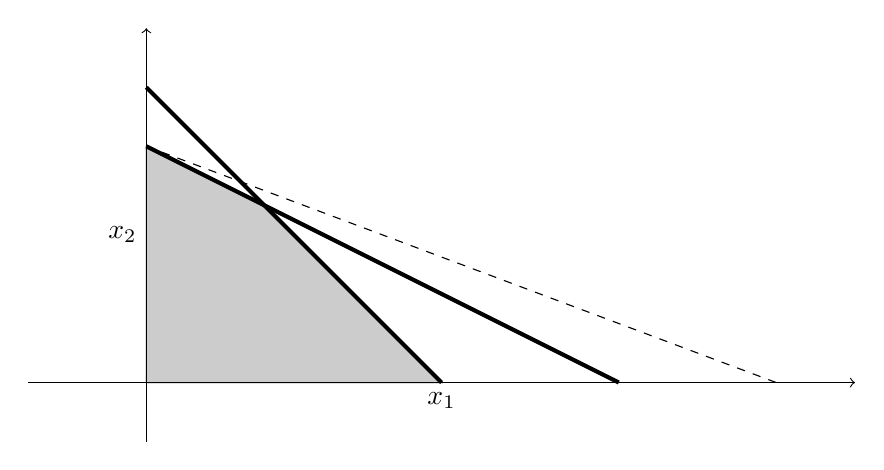
\begin{tikzpicture}[x=1.5cm, y=0.75cm]
                        \draw[fill=black!20] (0, 0) -- (0, 4) -- (1, 3) -- (2.5, 0) -- cycle;
                        \draw
                        (0, 4) edge[dashed] (16/3, 0)
                        (0, -1) edge[->, left] node{$x_2$} (0, 6)
                        (-1, 0) edge[->, below] node{$x_1$} (6, 0)
                        (0, 4) edge[line width=1.5pt] (4, 0)
                        (0, 5) edge[line width=1.5pt] (2.5, 0);
                    \end{tikzpicture}
                \end{center}
                We then want to convert this into standard form as follows;
                \begin{mini*}|l|
                    {}{z = -3x_1 - 4x_2}
                    {}{-}
                    \addConstraint{x_1 + x_2 + x_3}{= 4}
                    \addConstraint{2x_1 + x_2 + x_4}{= 5}
                    \addConstraint{x_1, x_2, x_3, x_4}{\geq 0}
                \end{mini*}
                From this, we have 4 columns, and let us choose our index set $I = \{1, 2\}$.
                Therefore;
                \begin{align*}
                    \mat{B} & = \begin{bmatrix}
                        1 & 1 \\
                        2 & 1
                    \end{bmatrix} \\
                    \mat{B}^{-1} & = \begin{bmatrix}
                        -1 & 1 \\
                        2 & -1
                    \end{bmatrix} \\
                    \vec{x_B} & = \mat{B}^{-1}\vec{b} \\
                    & = \begin{bmatrix}
                        -1 & 1 \\
                        2 & -1
                    \end{bmatrix} \begin{bmatrix}
                        4 \\ 5
                    \end{bmatrix} \\
                    & = \begin{bmatrix}
                        1 \\ 3
                    \end{bmatrix} \\
                    \vec{x} & = \begin{bmatrix}
                        1 \\ 3 \\ 0 \\ 0
                    \end{bmatrix} & \text{this is a basic feasible solution}
                \end{align*}
                With a fixed index set $I$ where $|I| = m$ and $B(I)$ invertible.
                The variables $\{x_i\}_{i \in I}$ are referred to as basic variables, while the other variables $\{x_i\}_{i \notin I}$ are referred to as the nonbasic variables corresponding to $I$.
                Nonbasic variables are \textbf{always} zero, but the basic variables can be anything (including zero).
                \medskip

                The \textbf{basic representation} corresponding to $I$ is the unique reformulation of the system $z = \vec{c}^\top\vec{x}$ and $\mat{A}\vec{x} = \vec{b}$, which expresses the objective function value $z$ and each basic variable as a linear function of the nonbasic variables;
                $$\begin{bmatrix}
                    z \\ \vec{x_B}
                \end{bmatrix} = f(\vec{x_N})$$
                \begin{itemize}
                    \itemsep0em
                    \item $\vec{x_B} = [x_i\ \vline\ i \in I]$ (basic variable)
                    \item $\vec{x_N} = [x_i\ \vline\ i \notin I]$ (nonbasic variable)
                    \item $f : \mathbb{R}^{n - m} \to \mathbb{R}^{m + 1}$ is \textbf{linear}
                \end{itemize}
                Once again, let $\mat{A} = [\vec{a_1}, \dots, \vec{a_n}]$. where $\vec{a_i} \in \mathbb{R}^m$ is the $i^\text{th}$ column of $\mat{A}$.
                Take any index set $I \subseteq \{1, \dots, m\}$ with $|I| = m$, we can define the following;
                \begin{align*}
                    \mat{B} & = [\vec{a_i}\ \vline\ i \in I] \\
                    \mat{N} & = [\vec{a_i}\ \vline\ i \notin I] \\
                    \vec{c_B} & = [c_i\ \vline\ i \in I] \\
                    \vec{c_N} & = [c_i\ \vline\ i \notin I] \\
                    \vec{x_B} & = [x_i\ \vline\ i \in I] \\
                    \vec{x_N} & = [x_i\ \vline\ i \notin I] \\
                    \intertext{This implies that;}
                    \mat{A}\vec{x} & = \mat{B}\vec{x_B} + \mat{N}\vec{x_N} \\
                    \vec{c}^\top\vec{x} & = \vec{c_B}^\top\vec{x_B} + \vec{c_N}^\top\vec{x_N}
                \end{align*}
                Given this partition, we have the following;
                $$\left.\begin{aligned}
                    z & = \vec{c}^\top\vec{x} \\
                    \mat{A}\vec{x} & = \vec{b}
                \end{aligned}\right\rbrace \Leftrightarrow \left\lbrace\begin{aligned}
                    z & = \vec{c_B}^\top\vec{x_B} + \vec{c_N}^\top\vec{x_N} \\
                    \mat{B}\vec{x_B} & = \vec{b} - \mat{N}\vec{x_N}
                \end{aligned}\right.$$
                Since $\mat{B}$ is invertible, we can get the following;
                \begin{align*}
                    \vec{x_B} & = \mat{B}^{-1}(\vec{b} - \mat{N}\vec{x_N}) \\
                    & = \mat{B}^{-1}\vec{b} - \mat{B}^{-1}\mat{N}\vec{x_N} \\
                    z & = \vec{c_B}^\top\vec{x_B} + \vec{c_N}^\top\vec{x_N} \\
                    & = \vec{c_B}^\top(\mat{B}^{-1}\vec{b} - \mat{B}^{-1}\mat{N}\vec{x_N}) + \vec{c_N}^\top\vec{x_N} \\
                    & = \vec{c_B}^\top\mat{B}^{-1}\vec{b} + (\vec{c_N}^\top - \vec{c_B}^\top\mat{B}^{-1}\mat{N})\vec{x_N} \\
                    & = \vec{c_B}^\top\mat{B}^{-1}\vec{b} + (\vec{c_N} - \mat{N}^\top\mat{B}^{-\top}\vec{c_B})^\top\vec{x_N} & \text{where } \mat{B}^{-\top} = (\mat{B}^{-1})^\top
                \end{align*}
                Therefore, the basic representation is as follows;
                \begin{align*}
                    z & = \vec{c_B}^\top\mat{B}^{-1}\vec{b} + (\vec{c_N} - \mat{N}^\top\mat{B}^{-\top}\vec{c_B})^\top\vec{x_N} \\
                    \vec{x_B} & = \mat{B}^{-1}\vec{b} - \mat{B}^{-1}\mat{N}\vec{x_N}
                \end{align*}
                This expresses $z$ and $\vec{x_B}$ as linear functions of $\vec{x_N}$.
                However by setting $\vec{x_N} = \vec{0}$, we obtain the basic solution $\vec{x} = (\vec{x_B}, \vec{x_N}) = (\mat{B}^{-1}\vec{b}, \vec{0})$, with the objective value $z = \vec{c_B}^\top\mat{B}^{-1}\vec{b}$.
                The \textbf{reduced cost vector} is $\vec{r} = \vec{c_N} - \mat{N}^\top\mat{B}^{-\top}\vec{c_B}$, which characterises the sensitivity of the objective function value $z$ with respect to the nonbasic variables.
                \medskip

                Referring back to the previous example;
                \begin{mini*}|l|
                    {}{z = -3x_1 - 4x_2}
                    {}{-}
                    \addConstraint{x_1 + x_2 + x_3}{= 4}
                    \addConstraint{2x_1 + x_2 + x_4}{= 5}
                    \addConstraint{x_1, x_2, x_3, x_4}{\geq 0}
                \end{mini*}
                Consider the solution we get when;
                \begin{align*}
                    I & = \{3, 4\} \\
                    O & = (0, 0, 4, 5) \\
                    z & = -3x_1 - 4x_2 \\
                    x_3 & = 4 - x_1 - x_2 \\
                    x_4 & = 5 - 2x_1 - x_2
                \end{align*}
                However, by looking at the objective function, we can see that it is more desirable to increase the value of $x_2$, so we fix $x_1 = 0$.
                This then gives us the following;
                \begin{align*}
                    z & = -4x_2 \\
                    x_3 & = 4 - x_2 \\
                    & \geq 0 \\
                    x_4 & = 5 - x_2 \\
                    & \geq 0 & \Rightarrow \\
                    x_2 & \leq 4 & \Rightarrow \\
                    x_2 & = 4 & \Rightarrow \\
                    x_3 & = 0
                \end{align*}
                This \textbf{pivoting} changes the index set to be $I = \{2, 4\}$.
                Looking at the nonbasic variables $\{x_1, x_3\}$;
                \begin{align*}
                    z & = -3x_1 - 4x_2 \\
                    & = -3x_1 - 4(\red{4 - x_1 - x_3}) \\
                    & = -3x_1 - 16 + 4x_1 + 4x_3 \\
                    & = -16 + x_1 + 4x_3 \\
                    \red{x_2} & = \red{4 - x_1 - x_3}
                \end{align*}
                We can see, by looking at the coefficients, that $x_1$ and $x_3$ will cause the minimal solution to increase if they weren't zero.
        \subsection*{Lecture 4}
            \subsubsection*{Simplex Tableau}
                If we consider a basic representation of the following form, where the reduced cost vector $\vec{r} = \vec{c_N} - \mat{N}^\top\mat{B}^{-\top}\vec{c_B}$;
                \begin{align*}
                    z - \vec{r}^\top\vec{x_N} & = \vec{c_B}^\top\mat{B}^{-1}\vec{b} \\
                    \vec{x_B} + \mat{B}^{-1}\mat{N}\vec{x_N} & = \mat{B}^{-1}\vec{b}
                \end{align*}
                We can represent it in the following \textbf{tableau};
                \begin{center}
                    \begin{tabular}{c|ccc|c}
                        BV & $z$ & $\vec{x_B}^\top$ & $\vec{x_N}^\top$ & RHS \\
                        \hline
                        $z$ & 1 & $\vec{0}^\top$ & $-\vec{r}^\top$ & $\vec{c_B}^\top\mat{B}^{-1}\vec{b}$ \\
                        $\vec{x_B}$ & $\vec{0}$ & $\mat{I}$ & $\mat{B}^{-1}\mat{N}$ & $\mat{B}^{-1}\vec{b}$
                    \end{tabular}
                \end{center}
                Note that here $\mat{I} \in \mathbb{R}^{m \times m}$ is an identity matrix.
                Also note the separation of the basic and non-basic variables for the tableau - typically we will simply write it in lexicographical order.
                If $\mat{B}^{-1}\vec{b} \geq 0$ then we can denote it as a BFS.
                \medskip

                Consider the previous example;
                \begin{align*}
                    z & = -3x_1 - 4x_2 \\
                    x_3 & = 4 - x_1 - x_2 \\
                    x_4 & = 5 - 2x_1 - x_2
                \end{align*}
                Note that the basic variables have a specific property where they are 0s in the columns, other than a 1 in its respective row;
                \begin{center}
                    \begin{tabular}{c|ccccc|c}
                        BV & $z$ & $x_1$ & $x_2$ & $x_3$ & $x_4$ & RHS \\
                        \hline
                        $z$ & 1 & 3 & 4 & 0 & 0 & 0 \\
                        $x_3$ & 0 & 1 & 1 & 1 & 0 & 4 \\
                        $x_4$ & 0 & 2 & 1 & 0 & 1 & 5
                    \end{tabular}
                \end{center}
                Consider the basic representation from the example, with the index set $I = \{1, 2, 5\}$, with the following explicit formulation;
                \begin{align*}
                    z - \frac{2}{5}x_3 - \frac{1}{5}x_4 & = -8 \\
                    x_2 - \frac{1}{5}x_3 + \frac{2}{5}x_4 & = 5 \\
                    -\frac{3}{5}x_3 + \frac{1}{5}x_4 + x_5 & = 1 \\
                    x_1 + \frac{3}{5}x_3 - \frac{1}{5}x_4 & = 3
                \end{align*}
                This can now be set in the tableau as;
                \begin{center}
                    \begin{tabular}{c|cccccc|c}
                        BV & $z$ & $x_1$ & $x_2$ & $x_3$ & $x_4$ & $x_5$ & RHS \\
                        \hline
                        $z$ & 1 & 0 & 0 & $-\frac{2}{5}$ & $-\frac{1}{5}$ & 0 & -8 \\
                        $x_2$ & 0 & 0 & 1 & $-\frac{1}{5}$ & $\frac{2}{5}$ & 0 & 5 \\
                        $x_5$ & 0 & 0 & 0 & $-\frac{3}{5}$ & $\frac{1}{5}$ & 1 & 1 \\
                        $x_1$ & 0 & 1 & 0 & $\frac{3}{5}$ & $-\frac{1}{5}$ & 0 & 3
                    \end{tabular}
                \end{center}
                The tableau is a practical way to analyse the basic solution associated to the basic representation;
                \begin{itemize}
                    \itemsep0em
                    \item the RHS of the objective row is the objective \textbf{value} of the current basic solution
                    \item the RHS's of the other rows are the values of the basic variables at the current basic solution
                    \item the coefficients of the non-basic variables in the \textbf{objective row} are the \textbf{negative reduced costs}
                    \item the current basic solution is feasible iff all the RHS's are $\geq 0$ (but the objective row can be negative)
                \end{itemize}
                The general tableau for a feasible index set $I$, with $p \in I, q \notin I$;
                \begin{center}
                    \begin{tabular}{c|cccccccc|c}
                        BV & $z$ & $x_1$ & $\cdots$ & $x_p$ & $\cdots$ & $x_q$ & $\cdots$ & $x_n$ & RHS \\
                        \hline
                        $z$ & 1 & $\beta_1$ & $\cdots$ & $\beta_p \violet{(= 0)}$ & $\cdots$ & $\beta_q$ & $\cdots$ & $\beta_n$ & $\beta_0$ \\
                        $\vdots$ & $\vdots$ & $\vdots$ & & $\vdots$ & & $\vdots$ & & $\vdots$ & $\vdots$ \\
                        $x_p$ & 0 & $y_{p, 1}$ & $\cdots$ & $y_{p, p}$ & $\cdots$ & $y_{p, q}$ & $\cdots$ & $y_{p, n}$ & $y_{p, 0}$ \\
                        $\vdots$ & $\vdots$ & $\vdots$ & & $\vdots$ & & $\vdots$ & & $\vdots$ & $\vdots$ \\
                        \hline
                    \end{tabular}
                \end{center}
                This has the following properties;
                \begin{itemize}
                    \itemsep0em
                    \item $\forall i \in I\ y_{i, i} = 1$, and $\forall i \in I, j \in I \setminus \{i\}\ y_{j, i} = 0$
                    \item $\forall i \notin I, i \neq 0\ \beta_i = -r_i$ \hfill negative reduced cost
                    \item $\forall i \in I\ \beta_i = 0$
                \end{itemize}
            \subsubsection*{Pivoting}
                The idea of the Simplex algorithm is that if a vertex $x$ for the index set $I$ is not optimal, then one of its neighbouring vertices will have a \textbf{better objective value}.
                Neighbouring are obtained by swapping a basic variable $x_p$ with a non-basic variable $x_q$, to obtain a new index set $I^\prime$ - $x_p$ \textbf{leaves} the basis and $x_q$ \textbf{enters} the basis.
                The technique called \textbf{pivoting} is used to efficiently compute the new basic representation by updating $I$ to $I^\prime$.
                This is similar to applying elementary row operations in Gaussian elimination, and the pair $(p, q)$ is referred to as the \textbf{pivot}.
                \medskip

                While it's possible to pivot to something that isn't feasible, in this algorithm we will only look at pivots to feasible solutions.
                Consider the following, starting with the basic solution for the index set $I = \{1, 2, 4\}$;
                \begin{center}
                    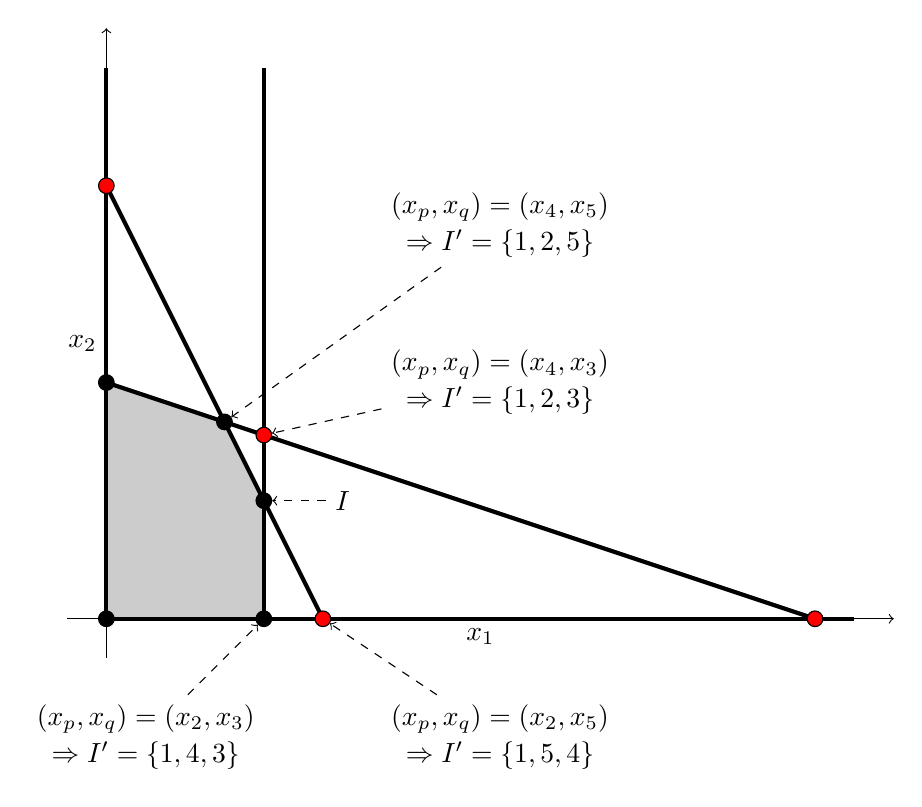
\begin{tikzpicture}[x=0.5cm, y=0.5cm]
                        \draw
                        (0, -1) edge[->, left] node{$x_2$} (0, 15)
                        (-1, 0) edge[->, below] node{$x_1$} (20, 0);

                        \draw[fill=black!20] (0, 0) -- (0, 6) -- (3, 5) -- (4, 3) -- (4, 0) -- cycle;

                        \draw
                        (0, 0) edge[line width=1.5pt] (0, 14)
                        (0, 0) edge[line width=1.5pt] (19, 0)
                        (0, 11) edge[line width=1.5pt] (5.5, 0)
                        (0, 6) edge[line width=1.5pt] (18, 0)
                        (4, 0) edge[line width=1.5pt] (4, 14);

                        \node[rbtb] (a) at (0, 0) {};
                        \node[rbtb] (b) at (0, 6) {};
                        \node[rbtb] (c) at (3, 5) {};
                        \node[rbtb] (d) at (4, 3) {};
                        \node[rbtb] (e) at (4, 0) {};

                        \node[rbtr] (f) at (0, 11) {};
                        \node[rbtr] (g) at (4, 14/3) {};
                        \node[rbtr] (h) at (5.5, 0) {};
                        \node[rbtr] (i) at (18, 0) {};

                        \node (bsi) at (6, 3) {$I$};
                        \node (bsig) at (10, 6) {\shortstack{$(x_p, x_q) = (x_4, x_3)$\\$\Rightarrow I^\prime = \{1, 2, 3\}$}};
                        \node (bsih) at (10, -3) {\shortstack{$(x_p, x_q) = (x_2, x_5)$\\$\Rightarrow I^\prime = \{1, 5, 4\}$}};
                        \node (bsie) at (1, -3) {\shortstack{$(x_p, x_q) = (x_2, x_3)$\\$\Rightarrow I^\prime = \{1, 4, 3\}$}};
                        \node (bsic) at (10, 10) {\shortstack{$(x_p, x_q) = (x_4, x_5)$\\$\Rightarrow I^\prime = \{1, 2, 5\}$}};

                        \draw
                        (bsi) edge[->, dashed] (d)
                        (bsig) edge[->, dashed] (g)
                        (bsih) edge[->, dashed] (h)
                        (bsie) edge[->, dashed] (e)
                        (bsic) edge[->, dashed] (c);
                    \end{tikzpicture}
                \end{center}
                In order to swap $x_p$ and $x_q$ we perform the following steps;
                \begin{enumerate}[1.]
                    \itemsep0em
                    \item \textbf{divide} row $p$ by the pivot element $y_{p, q}$ and relabel it as row $q$;
                        $$\forall j = 0, \dots, n\ \left[y^\prime_{q, j} = \frac{y_{p, j}}{y_{p, q}}\right]$$
                    \item \textbf{subtract} row $p$ multiplied by $\frac{y_{i, q}}{y_{p, q}}$ from row $i \in I \setminus \{p\}$
                        $$\forall j = 0, \dots, n\ \left[y^\prime_{i, j} = y_{i, j}  \frac{y_{i, q}}{y_{p, q}}y_{p, j}\right]$$
                    \item \textbf{subtract} row $p$ multiplied by $\frac{\beta_q}{y_{p, q}}$ from the objective row
                        $$\forall j = 0, \dots, n\ \left[\beta^\prime_j = \beta_j - \frac{\beta_q}{y_{p, q}}y_{p, j}\right]$$
                \end{enumerate}
                Applying the following steps to the example table (note that a new horizontal line denotes a new table).
                Note that we are swapping out $x_4$ for $x_1$, hence $y_{p, q} = y_{4, 1} = 2$;
                \begin{center}
                    \begin{tabular}{c|ccccc|c}
                        BV & $z$ & $x_1$ & $x_2$ & $x_3$ & $x_4$ & RHS \\
                        \hline
                        $z$ & 1 & 3 & 4 & 0 & 0 & 0 \\
                        $x_3$ & 0 & 1 & 1 & 1 & 0 & 4 \\
                        $x_4$ & 0 & 2 & 1 & 0 & 1 & 5 \\
                        \hline
                        $z$ & 1 & 0 & $\frac{5}{2}$ & 0 & $-\frac{3}{2}$ & $-\frac{15}{2}$ \\
                        $x_3$ & 0 & 0 & $\frac{1}{2}$ & 1 & $-\frac{1}{2}$ & $\frac{3}{2}$ \\
                        $x_4$ & 0 & 1 & $\frac{1}{2}$ & 0 & $\frac{1}{2}$ & $\frac{5}{2}$ \\
                    \end{tabular}
                \end{center}
                Note that both the RHS's of the basic variables are non-negative, hence we have a BFS.
                However, since there are positive coefficients for the nonbasic variables in the objective row, we can still improve this value.
                \medskip

                We need a way to choose the variable $x_q$, which enters the basis.
                Consider that the objective row is equivalent to;
                $$z + \summation{i = 1}{n} \beta_i x_i = \beta_0 \Leftrightarrow z = \beta_0 - \summation{i \notin I}{} \beta_i x_i$$
                We also know the following, by definition;
                $$\beta_i = \begin{cases}
                    0 & \text{if } i \in I \text{\hspace{20pt} (basic variables)} \\
                    -r_i & \text{if } i \notin I \text{\hspace{20pt} (nonbasic variables)}
                \end{cases}$$
                Any nonbasic $x_i$ with $\beta_i > 0$ can enter the basis and become $x_q$, since each of them will decrease $z$, however, we can use the following steps to choose one;
                \begin{itemize}
                    \itemsep0em
                    \item if there only exists a single $x_i$ with $\beta_i > 0$, pick this as $x_q$
                    \item if several $x_i$ have $\beta_i > 0$, pick $x_i$ with \textbf{largest} $\beta_i$
                    \item if several $x_i$ have the same largest $\beta_i$, pick the \textbf{smallest} index $x_i$
                \end{itemize}
                Similarly, we also need to choose which basic variable $x_p$ to leave the basis.
                We need to ensure the following for all variables $x_i$ in the index set $I$;
                $$x_i = y_{i, 0} - y_{i, q} x_q \geq 0 \Leftrightarrow \begin{cases}
                    x_q \leq \bar{x}_{i, q} \triangleq \dfrac{y_{i, 0}}{y_{i, q}}& \text{if } y_{i, q} > 0 \\
                    x_q \leq \bar{x}_{i, q} \triangleq \infty & \text{if } y_{i, q} \leq 0 \\
                \end{cases}$$
                This means that if $y_{i, q}$ is positive, we have an upper bound, however if it's negative (or zero), it is unbounded (hence $\infty$).
                For this to be feasible, we want to ensure that $x_q$ is set such that all bounds are simultaneously satisfied;
                $$x_q \leq \min_{i \in I} \bar{x}_{i, q}$$
                There are two cases for picking the variable $x_p$ to leave the basis;
                \begin{itemize}
                    \itemsep0em
                    \item \textbf{trivial bounds} ($\min_{i \in I} \bar{x}_{i, q} = \infty$)
                        \smallskip

                        In this case, the entering variables $x_q$ can grow indefinitely.
                        Since we have $\beta_q > 0$, the objective value $z = \beta_0 - \beta_q x_q$ can drop indefinitely, hence the LP is unbounded.
                        In this case, we don't need to choose an $x_p$ variable.
                    \item \textbf{non-trivial}
                        \smallskip

                        Here the best value of the objective is obtained by maximising $x_q$, hence setting;
                        $$x_q = \min_{i \in I} \bar{x}_{i, q}$$
                        We can call $p$ the row such that $\bar{x}_{p, q} = \min_{i \in I} \bar{x}_{i, q}$, which is the row that constraints the most the increase in value of $x_q$.
                        Similarly, if there are multiple $p$ satisfying this, we can choose the one with the smallest index.
                \end{itemize}
                In summary, the simplex algorithm (minimisation) is as follows;
                \begin{enumerate}[1.]
                    \setcounter{enumi}{-1}
                    \itemsep0em
                    \item find initial BFS and its basic representation
                    \item if $\beta_i \leq 0$ for all $i \notin I$; we can stop, the current BFS is optimal
                    \item if $\exists j \notin I$ with $\beta_j > 0$ and $y_{i, j} \leq 0$ for all $i \in I$; we can stop, no finite minimum exists
                    \item choose $x_q$ with the largest $\beta_q > 0$ ($x_q$ enters the basis)
                    \item choose $p \in \argmin_{i \in I} \bar{x}_{i, q}$ ($x_p$ leaves the basis)
                    \item pivot on $y_{p, q}$ and repeat from step 1
                \end{enumerate}
                In the example below, I will denote the $\beta_i$ chosen for $x_q$ in \violet{violet}, the pivot in \teal{teal}, and calculations for $\bar{x}_{i, q}$ in \blue{blue}.
                \begin{center}
                    \begin{tabular}{c|ccccc|c}
                        BV & $z$ & $x_1$ & $x_2$ & $x_3$ & $x_4$ & RHS \\
                        \hline
                        $z$ & 1 & 3 & \violet{4} & 0 & 0 & 0 \\
                        $x_3$ & 0 & 1 & \teal{1} & 1 & 0 & 4 \blue{$\frac{4}{1} = \bar{x}_{3, 2}$} \\
                        $x_4$ & 0 & 2 & 1 & 0 & 1 & 5 \blue{$\frac{5}{1} = \bar{x}_{4, 2}$} \\
                        \hline
                        $z$ & 1 & $-1$ & 0 & $-4$ & 0 & $-16$ \\
                        $x_2$ & 0 & 1 & 1 & 1 & 0 & 4 \\
                        $x_4$ & 0 & 1 & 0 & $-1$ & 1 & 1 \\
                    \end{tabular}
                \end{center}
                Note that both the coefficients are negative in the objective row, we have the following optimal solution;
                \begin{align*}
                    z^* & = -16 \\
                    y^* & = 16 \\
                    x^* & = (0, 4, 0, 1)
                \end{align*}
            \subsubsection*{Tutorial}
                \begin{enumerate}[1.]
                    \itemsep0em
                    \setcounter{enumi}{1}
                    \item Consider the following optimisation problem;
                        \begin{maxi*}|l|
                            {}{y = x_1 + 3x_2}
                            {}{}
                            \addConstraint{2x_1 + x_2}{\leq 4}
                            \addConstraint{x_1 + 2x_2}{\leq 4}
                            \addConstraint{x_1, x_2}{\geq 0}
                        \end{maxi*}
                        \begin{enumerate}[(a)]
                            \item Bring the problem into standard form by introducing slack variables $s_1$ and $s_2$.
                                \begin{mini*}|l|
                                    {}{z = -x_1 - 3x_2}
                                    {}{-}
                                    \addConstraint{2x_1 + x_2 + s_1}{= 4}
                                    \addConstraint{x_1 + 2x_2 + s_2}{= 4}
                                    \addConstraint{x_1, x_2, s_1, s_2}{\geq 0}
                                \end{mini*}
                            \item
                                For the problem in standard form, determine all basic solutions.
                                Which of these problems are feasible, and what are their objective values?
                                \begin{align*}
                                    \text{BV} & = \{x_1, x_2\} \\
                                    \text{NBV} & = \{s_1, s_2\} \\
                                    2x_1 + x_2 & = 4 \\
                                    x_1 + 2x_2 & = 4 \\
                                    -3x_1 & = -4 & \Rightarrow \\
                                    x_1 & = \frac{4}{3} & \Rightarrow \\
                                    x_2 & = \frac{4}{3} & \Rightarrow \\
                                    D & = \left(\frac{4}{3}, \frac{4}{3}, 0, 0\right) & \text{feasible} \\
                                    z & = -\frac{16}{3} \\ \\
                                    \text{BV} & = \{x_2, s_1\} \\
                                    \text{NBV} & = \{x_1, s_2\} \\
                                    x_2 + s_1 & = 4 \\
                                    2x_2 & = 4 \\
                                    x_2 & = 2 & \Rightarrow \\
                                    s_1 & = 2 & \Rightarrow \\
                                    D & = (0, 2, 2, 0) & \text{feasible} \\
                                    z & = -6
                                \end{align*}
                            \item
                                Draw the feasible region of problem 1 in the $(x_1,x_2)$-plane.
                                Where are the basic solutions from part (b)?
                                Which feasible solutions satisfy $s_1 = 0$?
                                Which feasible solutions satisfy $s_2 = 0$?

                                \begin{center}
                                    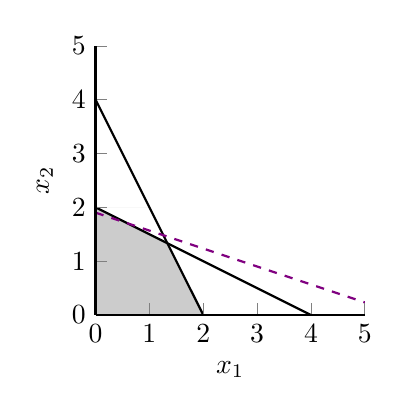
\begin{tikzpicture}
                                        \begin{axis}[
                                            axis on top=true,
                                            axis line style=thick,
                                            no markers, domain=0:8, samples=10,
                                            axis lines*=left, xlabel=$x_1$, ylabel=$x_2$,
                                            height=5cm, width=5cm,
                                            enlargelimits=false,
                                            xtick={0,1,...,5},
                                            ytick={0,1,...,5},
                                            xmin=0, xmax=5,
                                            ymin=0, ymax=5
                                        ]
                                            \addplot[fill=black!20, draw=none] {1.995} \closedcycle;

                                            \addplot[fill=white!20, draw=none] {4 - 2*\x} |- (current plot begin);
                                            \addplot[fill=white!20, draw=none] {2 - 0.5*\x} |- (current plot begin);

                                            \addplot[thick] {4 - 2*\x};
                                            \addplot[thick] {2 - 0.5*\x};

                                            \addplot[thick, dashed, violet] {1.9 - \x/3};
                                        \end{axis}
                                    \end{tikzpicture}
                                \end{center}
                        \end{enumerate}
                    \item Consider the basic solution from exercise 2 (b) that has $x_1$ and $x_2$ as basic variables.
                        \begin{enumerate}[(a)]
                            \itemsep0em
                            \item Determine the basic representation for this basic solution.
                            \item
                                Is this basic solution optimal?
                                Justify your answer both graphically (see exercise 2 (c)) and from the basic representation.
                            \item
                                Find a non-basic variable such that increasing its value improves the objective value.
                                How much can we increase the value of this basic variable without leaving the feasible region?
                                Which is the resulting basic solution?
                                Is this solution optimal?
                        \end{enumerate}
                \end{enumerate}
        \subsection*{Lecture 5}
            \subsubsection*{Degenerate Basic Solutions}
                Consider a variation of our first example, where the $x \leq 4$ constraint has changed to $x \leq 3$.
                One property we can quickly see is that there are now three lines intersecting a specific point $(3, 5)$, compared to the two of standard points.
                Essentially, the coordinates of this point are determined by more constraints than strictly necessary, and the three index sets that would typically identify different points now identify the same point.
                This can cause some of the basic variables to also be set to zero, in this case $x_3 = x_4 = x_5 = 0$.
                \begin{center}
                    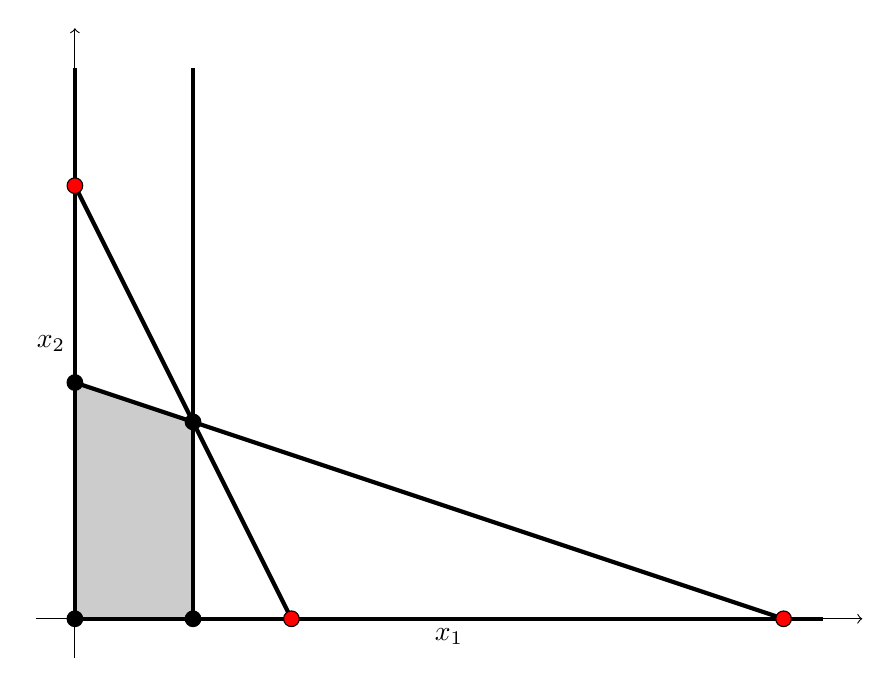
\begin{tikzpicture}[x=0.5cm, y=0.5cm]
                        \draw
                        (0, -1) edge[->, left] node{$x_2$} (0, 15)
                        (-1, 0) edge[->, below] node{$x_1$} (20, 0);

                        \draw[fill=black!20] (0, 0) -- (0, 6) -- (3, 5) -- (3, 0) -- cycle;

                        \draw
                        (0, 0) edge[line width=1.5pt] (0, 14)
                        (0, 0) edge[line width=1.5pt] (19, 0)
                        (0, 11) edge[line width=1.5pt] (5.5, 0)
                        (0, 6) edge[line width=1.5pt] (18, 0)
                        (3, 0) edge[line width=1.5pt] (3, 14);

                        \node[rbtb] (a) at (0, 0) {};
                        \node[rbtb] (b) at (0, 6) {};
                        \node[rbtb] (c) at (3, 5) {};
                        \node[rbtb] (e) at (3, 0) {};

                        \node[rbtr] (f) at (0, 11) {};
                        \node[rbtr] (h) at (5.5, 0) {};
                        \node[rbtr] (i) at (18, 0) {};
                    \end{tikzpicture}
                \end{center}
                We can define a basic solution as \textbf{degenerate} if one or more basic variables are zero.
                This means that a degenerate basic solution has more than $n - m$ zero-valued variables, therefore if we look at the tableau, there exists at least a basic variable such that $i \in I$ and $y_{i, 0} = 0$.
                \medskip

                On the other hand, we can define a basic solution as \textbf{non-degenerate} if all of its basic variables are different from zero.
            \subsubsection*{Finite Termination Theorem}
                The theorem states that if all basic feasible solutions are \textbf{non-degenerate}, then the simplex algorithm must terminate after a \textbf{finite} number of steps, either with an optimal solution, or a proof that the problem is unbounded.
                The proof is as follows;
                \begin{itemize}
                    \itemsep0em
                    \item Due to non-degeneracy, we have $\forall i \in I\ [y_{i, 0} > 0]$
                    \item Unless we find an optimal solution, or detect unboundedness in steps 1 or 2, we have;
                        $$\beta^\prime_0 = \beta_0 - \frac{\beta_q}{y_{p, q}}y_{p_0} < \beta_0$$
                        Looking at the signs, we know that $\beta_q > 0$ (from how we choose the variable $x_q$ entering the basis).
                        Similarly, we know that $y_{p, q} > 0$, otherwise we have an unbounded LP (since we choose the minimum value, and if all the bounds are $\infty$, we will encounter the unbounded case).
                        Finally, we also know that $y_{p, 0}$ must also be positive, hence the entire product is strictly positive.
                    \item As such, we have a strictly decreasing sequence of objective values;
                        $$\beta_0 > \beta^\prime_0 > \beta^{\prime\prime}_0 > \dots$$
                        This results in no basic solution being repeated.
                    \item Since there are $\binom{n}{m}$ ways to pick $m$ columns out of $n$ to form an index set $I$, we can say that there are $\leq \binom{n}{m}$ basic solutions
                    \item As such, the process cannot continue indefinitely and must terminate at either step 1 or 2 after a finite number of iterations
                \end{itemize}
            \subsubsection*{Degeneracy}
                We have the following lemma; assuming that $\forall i \in [1, n]$, there exists a basic solution $\hat{x}$, with $\hat{x}_i \neq 0$.
                Then a basic solution $x$ is \textbf{degenerate} iff it is associated with \textbf{more than one index set}.
                The proof is as follows (proving that if the basic solution $x$ has more than one index set $\Rightarrow$ the basic solution $x$ is degenerate);
                \begin{itemize}
                    \itemsep0em
                    \item Suppose $x$ corresponds to the index sets $I_1$ and $I_2$, where $I_1 \neq I_2$
                    \item Then $x_i = 0$ for all nonbasic variables $x_i$, and $i \notin I_1$, $i \notin I_2$ (or both)
                    \item Since $I_1 \neq I_2$, there must be a nonbasic variable $x_i$ in $I_1$, which is a basic variable in $I_2$, and since the two sets describe the same basic solution $x$, $x_i$ must be 0 in $I_2$ where it is basic (note that this also holds the other way around)
                    \item Therefore, $x$ is a degenerate basic solution
                \end{itemize}
                For example, consider the basic solution $x$ corresponding to index sets $I_1 = \{1, 2, 3\}$ and $I_2 = \{1, 2, 4\}$.
                Therefore $x_4 = 0$ due to $I_1$, and $x_3 = 0$ due to $I_2$.
                \medskip

                The steps to prove the other direction of the implication (where a degenerate basic solution $x$ $\Rightarrow$ the basic solution has more than one index set) is as follows;
                \begin{itemize}
                    \itemsep0em
                    \item Consider the corresponding simplex tableau, where $x$ is a degenerate basic solution corresponding to the index set $I$
                    \item Due to degeneracy, we have $\exists p \in I\ [y_{p, 0} = 0]$
                    \item There must also $\exists q \notin I\ [y_{p, q} \neq 0]$, otherwise we would always have $x_p = 0$ in all the feasible set (impossible with the theorem statement)
                        \smallskip

                        Consider the following table;
                        \begin{center}
                            \begin{tabular}{c|ccccc|c}
                                BS & $\cdots$ & $x_p$ & $\cdots$ & $x_q$ & $\cdots$ & RHS \\
                                \hline
                                $x_p$ & $\cdots$ & 1 & $\cdots$ & $y_{p, q}$ & $\cdots$ & 0
                            \end{tabular}
                        \end{center}
                        Note that if $y_{p, q} = 0$ (such that the only non-zero element in the row is $y_{p, p} = 1$), we would have $x_p = 0$.
                    \item Since we know this exists, we can pivot on $(p, q)$, which gives a new basic solution;
                        $$\violet{y^\prime_{q, 0}} = \frac{y_{p, 0}}{y_{p, q}} = 0 = \violet{y_{p, 0}} \text{   and also   } \forall i \in I \setminus \{p\} \left[\teal{y^\prime_{i, 0}} = y_{i, 0} - \frac{y_{i, q}}{y_{p, q}}\violet{y_{p, 0}} = \teal{y_{i, 0}}\right]$$
                        This basic solution is identical to the current one
                    \item Therefore, $x$ corresponds to both the index set $I$ and $(I \setminus \{p\}) \cup \{q\}$
                \end{itemize}
                This breaks the finite termination of the simplex algorithm since;
                \begin{itemize}
                    \itemsep0em
                    \item The index sets $I$ and $(I \setminus \{p\}) \cup \{q\}$ produce the same basic feasible solution, but with different basic representations
                    \item If we pivot on $(p, q)$, when $y_{p, 0} = 0$, the new basic feasible solution is identical to the old one
                    \item Therefore, we have no strict monotonic improvement of the objective value since;
                        $$\violet{\beta^\prime_0} = \beta_0 - \frac{\beta_q}{y_{p, q}}y_{p, 0} = \beta_0 - \frac{\beta_q}{y_{p, q}}0 = \violet{\beta_0}$$
                    \item We denote a pivot step $(p, q)$ as \textbf{degenerate} if $y_{p, 0} = 0$, and \textbf{non-degenerate} otherwise
                \end{itemize}
                We can then decompose the simplex algorithm into a \violet{sequence of degenerate pivots}, followed by a non-degenerate pivot, followed by a \violet{sequence of degenerate pivots}.
                Note that some / all of these degenerate pivot sequences can be empty.
                Geometrically, the basic feasible solution remains unchanged through a sequence of degenerate pivots, and only moves to a different BFS on a non-degenerate pivot.
            \subsubsection*{Cycling}
                We know that there is a finite number of index sets if \textbf{no index set is repeated}, as the number of index sets is $\leq \binom{n}{m}$.
                However, pivoting can result in cycling behaviour in some rare instances.
                Generally, choosing degenerate pivots is a necessary condition, but not a sufficient one, for cycling.
                After a sequence of pivots we return to the same index set, causing cycling.
                \medskip

                Consider the following example;
                \begin{mini*}|l|
                    {}{z = -\frac{3}{4}x_4 + 20x_5 - \frac{1}{2}x_6 + 6x_7}
                    {}{}
                    \addConstraint{x_1 + \frac{1}{4}x_4 - 8x_5 - x_6 + 9x_7}{= 0}
                    \addConstraint{x_2 + \frac{1}{2}x_4 - 12x_5 - \frac{1}{2}x_6 + 3x_7}{= 0}
                    \addConstraint{x_3 + x_6}{= 1}
                \end{mini*}
                When $I = \{1, 2, 3\}$, we have the following tableau;
                \begin{center}
                    \begin{tabular}{c|ccccccc|c}
                        BV & $x_1$ & $x_2$ & $x_3$ & $x_4$ & $x_5$ & $x_6$ & $x_7$ & RHS \\
                        \hline
                        $z$ & 0 & 0 & 0 & $\frac{3}{4}$ & $-20$ & $\frac{1}{2}$ & $-6$ & 0 \\
                        $x_1$ & 1 & 0 & 0 & $\red{\frac{1}{4}}$ & $-8$ & $-1$ & 9 & 0 \\
                        $x_2$ & 0 & 1 & 0 & $\frac{1}{2}$ & $-12$ & $-\frac{1}{2}$ & 3 & 0 \\
                        $x_3$ & 0 & 0 & 1 & 0 & 0 & 1 & 0 & 1 \\
                        \hline
                        $z$ & $-3$ & 0 & 0 & 0 & 4 & $\frac{7}{2}$ & $-33$ & 0 \\
                        $x_4$ & 4 & 0 & 0 & 1 & $-32$ & $-4$ & 36 & 0 \\
                        $x_2$ & $-2$ & 1 & 0 & 0 & $\red{4}$ & $\frac{3}{2}$ & $-15$ & 0 \\
                        $x_3$ & 0 & 0 & 1 & 0 & 0 & 1 & 0 & 1 \\
                        \hline
                        $z$ & $-1$ & $-1$ & 0 & 0 & 0 & 2 & $-18$ & 0 \\
                        $x_4$ & $-12$ & 8 & 0 & 1 & 0 & $\red{8}$ & $-84$ & 0 \\
                        $x_5$ & $-\frac{1}{2}$ & $\frac{1}{4}$ & 0 & 0 & 1 & $\frac{3}{8}$ & $-\frac{15}{4}$ & 0 \\
                        $x_3$ & 0 & 0 & 1 & 0 & 0 & 1 & 0 & 1 \\
                        \hline
                        $z$ & 2 & $-3$ & 0 & $-\frac{1}{4}$ & 0 & 0 & 3 & 0 \\
                        $x_4$ & $-\frac{3}{2}$ & 1 & 0 & $\frac{1}{8}$ & 0 & 1 & -$\frac{21}{2}$ & 0 \\
                        $x_2$ & $\frac{1}{16}$ & $-\frac{1}{8}$ & 0 & $\frac{3}{64}$ & 1 & 0 & $\frac{3}{16}$ & 0 \\
                        $x_3$ & $\frac{3}{2}$ & $-1$ & 1 & $\frac{1}{8}$ & 0 & 0 & $\frac{21}{2}$ & 1 \\
                        \hline
                        \multicolumn{9}{c}{$\vdots$} \\
                        \hline
                        $z$ & 0 & 0 & 0 & $\frac{3}{4}$ & $-20$ & $\frac{1}{2}$ & $-6$ & 0 \\
                        $x_1$ & 1 & 0 & 0 & $\red{\frac{1}{4}}$ & $-8$ & $-1$ & 9 & 0 \\
                        $x_2$ & 0 & 1 & 0 & $\frac{1}{2}$ & $-12$ & $-\frac{1}{2}$ & 3 & 0 \\
                        $x_3$ & 0 & 0 & 1 & 0 & 0 & 1 & 0 & 1
                    \end{tabular}
                \end{center}
                We can avoid cycling by amending the pivoting convention.
                Bland's rule states the following (with this rule, the algorithm cannot cycle and is therefore finite);
                \begin{enumerate}[(i)]
                    \itemsep0em
                    \item choose the \textbf{lowest-numbered} (leftmost) nonbasic column $q$ with a positive cost (instead of choosing the largest $\beta$);
                        $$q = \min \{ j \neq 0\ \vline\ \beta_j > 0 \}$$
                    \item Denote as $p$ the row with minimal $\bar{x}_{i, q}$, choosing the smallest index in the case of a tie (same as standard convention)
                \end{enumerate}
            \subsubsection*{Degeneracy in Practice}
                More recent experience with larger problems indicates that cycling occurs (while still being a rare event).
                Remedies such as Bland's rule are not satisfactory as it increases the number of iterations (and therefore time) in problems where cycles do not occur.
                In practice, it's possible to introduce a small perturbation by \textbf{replacing} a $y_{i, 0} = 0$ with $y_{i, 0} = \epsilon > 0$, and continue from there.
        \subsection*{Lecture 6}
            \subsubsection*{Initial Basic Feasible Solution}
                In the initial step (step 0) of the simplex algorithm, we require an \textbf{initial} BFS and the corresponding basic representation.
                \medskip

                We can consider the ``all slack basis'';
                \begin{mini*}|l|
                    {}{z = c_1x_1 + c_2x_2 + \dots + c_nx_n}
                    {}{}
                    \addConstraint{a_{1, 1}x_1 + a_{1, 2}x_2 + \dots + a_{1, n}x_n + \red{x_{n + 1}}}{= b_1}
                    \addConstraint{a_{2, 1}x_1 + a_{2, 2}x_2 + \dots + a_{2, n}x_n + \red{x_{n + 2}}}{= b_2}
                    \addConstraint{\vdots}{}
                    \addConstraint{a_{m, 1}x_1 + a_{m, 2}x_2 + \dots + a_{m, n}x_n + \red{x_{n + m}}}{= b_m}
                    \addConstraint{x_1, \dots, x_n, \red{x_{n + 1}, \dots, x_{n + m}}}{\geq 0}
                \end{mini*}
                Therefore we can take a basic representation for $I = {n + 1, \dots, n + m}$, which is feasible of $\forall i \in [1, m]\ b_i \geq 0$.
                However, this is not always the case.
                \medskip

                If we now consider an example without an obvious initial BFS, a system with equalities and inequalities in both direction, assuming all variables and RHS's are non-negative;
                \begin{align*}
                    x_1 + x_2 + x_3 & = 10 \\
                    2x_1 - x_2 & \geq 2 \\
                    x_1 - 2x_2 + x_3 \leq 6 \\
                    x_1, x_2, x_3 & \geq 0
                \end{align*}
                We can now standardise it by adding slack variables and subtracting surplus variables.
                Note that here we denote \red{slack variables in red} and \blue{surplus variables in blue};
                \begin{align*}
                    x_1 + x_2 + x_3 & = 10 \\
                    2x_1 - x_2 - \blue{x_4} & = 2 \\
                    x_1 - 2x_2 + x_3 + \red{x_5} & \leq 6 \\
                    x_1, x_2, x_3, \blue{x_4}, \red{x_5} & \geq 0
                \end{align*}
                Here we have no basic feasible representation, since only slack variables behave like basic variables.
                Another approach to the above is to introduce \violet{artificial variables} to the original equalities and $\geq$ inequalities;
                \begin{align*}
                    x_1 + x_2 + x_3 + \violet{\xi_1} & = 10 \\
                    2x_1 - x_2 - \blue{x_4} + \violet{\xi_2} & = 2 \\
                    x_1 - 2x_2 + x_3 + \red{x_5} & \leq 6 \\
                    x_1, x_2, x_3, \blue{x_4}, \red{x_5}, \violet{\xi_1}, \violet{\xi_2} & \geq 0
                \end{align*}
                The artificial variables behave like basic variables, and therefore we have a basic feasible representation.
                However, this system is not equivalent to the original one - when the artificial variables are zero the set of solutions is the same, however when they are strictly positive we will have more solutions.
                If we can find a basic feasible solution such that $\xi_1, \xi_2 = 0$, then we have found a basic feasible solution for the original LP.
                \medskip

                To find such a solution, we solve the \textbf{auxiliary LP};
                \begin{mini*}|l|
                    {}{\zeta = \xi_1 + \xi_2}
                    {}{}
                    \addConstraint{x_1 + x_2 + x_3 + \xi_1}{= 10}
                    \addConstraint{2x_1 - x_2 - x_4 + \xi_2}{= 2}
                    \addConstraint{x_1 - x_2 + x_3 + x_5}{= 6}
                    \addConstraint{x_1, x_2, x_3, x_4, x_5, \xi_1, \xi_2}{\geq 0}
                \end{mini*}
                Clearly, the minimum value we can achieve for $\zeta$ is 0.
                The initial BFS for this LP is given by $\xi_1 = 10, \xi_2 = 2, x_5 = 6$.
                If we are able to minimise $\zeta$ to 0, we have a basic feasible solution for the original LP, and if not, we cannot satisfy the original LP (it is infeasible).
                \medskip

                However, we need a basic representation for the initial BFS.
                The objective function $\zeta = \xi_1 + \xi_2$ is expressed in terms of the basic variables.
                To express $\zeta$ as a function of the nonbasic variables we add all equations with artificial variables to the objective;
                \begin{align*}
                    \zeta - \xi_1 - \xi_2 & = 0 & (+) \\
                    x_1 + x_2 + x_3 + \xi_1 & = 10 & (+) \\
                    2x_1 - x_2 - x_4 + \xi_2 & = 2 & (=) \\
                    \zeta + 3x_1 + x_3 - x_4 & = 12
                \end{align*}
                This auxiliary LP is feasible and bounded by construction, therefore the algorithm must terminate in step 1 with an optimal BFS, in one of two cases;
                \begin{itemize}
                    \itemsep0em
                    \item $\zeta = 0$ - this implies $\xi_1 = \xi_2 = 0$, and the optimal BFS of the auxiliary LP is a BFS for the original LP
                    \item $\zeta > 0$ - the auxiliary LP has no feasible solution with $\xi_1 = \xi_2 = 0$, hence the original system has no BFS, therefore it is infeasible
                \end{itemize}
                We can solve the auxiliary LP as follows;
                \begin{center}
                    \begin{tabular}{c|ccccccc|c}
                        BV & $x_1$ & $x_2$ & $x_3$ & $x_4$ & $x_5$ & $\xi_1$ & $\xi_2$ & RHS \\
                        \hline
                        $\zeta$ & 3 & 0 & 1 & $-1$ & 0 & 0 & 0 & 12 \\
                        $\xi_1$ & 1 & 1 & 1 & 0 & 0 & 1 & 0 & 10 \\
                        $\xi_2$ & $\red{2}$ & $-1$ & 0 & $-1$ & 0 & 0 & 1 & 2 \\
                        $x_5$ & 1 & $-2$ & 1 & 0 & 1 & 0 & 0 & 6 \\
                        \hline
                        $\zeta$ & 0 & $\frac{3}{2}$ & 1 & $\frac{1}{2}$ & 0 & 0 & $-\frac{3}{2}$ & 9 \\
                        $\xi_1$ & 0 & $\red{\frac{3}{2}}$ & 1 & $\frac{1}{2}$ & 0 & 1 & $-\frac{1}{2}$ & 9 \\
                        $x_1$ & 1 & $-\frac{1}{2}$ & 0 & $-\frac{1}{2}$ & 0 & 0 & $\frac{1}{2}$ & 1 \\
                        $x_5$ & 0 & $-\frac{3}{2}$ & 1 & $\frac{1}{2}$ & 1 & 0 & $-\frac{1}{2}$ & 5 \\
                        \hline
                        $\zeta$ & 0 & 0 & 0 & 0 & 0 & $-1$ & $-1$ & 0 \\
                        $x_2$ & 0 & 1 & $\frac{2}{3}$ & $\frac{1}{3}$ & 0 & $\frac{2}{3}$ & $-\frac{1}{3}$ & 6 \\
                        $x_1$ & 1 & 0 & $\frac{1}{3}$ & $-\frac{1}{3}$ & 0 & $\frac{1}{3}$ & $\frac{1}{3}$ & 4 \\
                        $x_5$ & 0 & 0 & 2 & 1 & 1 & 1 & $-1$ & 14
                    \end{tabular}
                \end{center}
                Since we've now found an optimal solution, and confirmed that $\zeta = 0$ at this point, we have $I = \{2, 1, 5\}$ as a BFS for the original system.
                We can also take the basic representation and omit $\zeta, \xi_1, \xi_2$ for phase 2.
            \subsubsection*{Two Phase Simplex Algorithm}
                The first phase is as follows;
                \begin{enumerate}[1.]
                    \itemsep0em
                    \item modify the constraints so that all RHS's are non-negative (multiply by $-1$ if a constraint has a negative RHS)
                    \item identify all equality and $\geq$ constraints
                    \item standardise inequalities (add slacks for $\leq$, subtract excesses for $\geq$)
                    \item add artificial constraints $\xi_i$ to the constraints identified in step 2
                    \item let $\zeta$ be the sum of all artificial variables and derive the basic representation for $\zeta$
                    \item find the minimum of $\zeta$ using the simplex algorithm
                \end{enumerate}
                There are three cases for the second phase, the trivial of which is when $\zeta^* > 0$, from which we can state that the original LP is infeasible.
                However, for the non-trivial case (when all $\xi_i$ are nonbasic at optimality), we perform the following steps;
                \begin{enumerate}[1.]
                    \itemsep0em
                    \item remove all artificial columns from the optimal phase 1 tableau
                    \item derive the basic representation for $z$ (original objective) with respect to the optimal index set from phase 1
                    \item solve the original LP with the simplex algorithms, using the final basis of phase 1 as the initial basis of phase 2 - the optimal of phase 2 is the optimal of the original LP
                \end{enumerate}
                On the other hand, when there is at least one basic $\xi_i$ at optimality;
                \begin{enumerate}[1.]
                    \itemsep0em
                    \item as $\zeta^* = 0$, we can conclude all $\xi_i = 0$, and therefore we have some basic variables equal to zero
                    \item we have found a degenerate BFS for the original LP, and a basic representation for the auxiliary problem
                    \item since the BFS is degenerate, we can pivot on $y_{p, q} \neq 0$, corresponding to an artificial $\xi_p$ and original variable $x_q$, and keep $\zeta^* = 0$
                    \item all $\xi_i$ variables can therefore be removed from the basis, obtaining a BFS for the original LP
                \end{enumerate}
        \subsection*{Lecture 7}
            \subsubsection*{Example}
                We can modify the running example as follows;
                \begin{maxi*}|l|
                    {}{y = 3x_1 + 4x_2}
                    {}{}
                    \addConstraint{x_1 + x_2}{\leq 4}
                    \addConstraint{2x_1 + x_2}{\leq 5}
                    \addConstraint{x_2}{\geq 1}
                    \addConstraint{x_1, x_2}{\geq 0}
                \end{maxi*}
                We can first transform this into the standard form as follows (by adding slack variables and subtracting an excess variable), and then adding \violet{artificial variables};
                \begin{mini*}|l|
                    {}{z = -3x_1 - 4x_2}
                    {}{-}
                    \addConstraint{x_1 + x_2 + x_3}{= 4}
                    \addConstraint{2x_1 + x_2 + x_4}{= 5}
                    \addConstraint{x_2 - x_5 + \violet{x_6}}{= 1}
                    \addConstraint{x_1, x_2, x_3, x_4, x_5, \violet{x_6}}{\geq 0}
                \end{mini*}
                This forms the auxiliary LP, where we can take the initial index set $I = \{3, 4, 6\}$;
                \begin{mini*}|l|
                    {}{\zeta = x_6}
                    {}{}
                    \addConstraint{x_1 + x_2 + x_3}{= 4}
                    \addConstraint{2x_1 + x_2 + x_4}{= 5}
                    \addConstraint{x_2 - x_5 + x_6}{= 1}
                    \addConstraint{x_1, x_2, x_3, x_4, x_5, x_6}{\geq 0}
                \end{mini*}
                We can now form the following simplex tableau (for phase 1);
                \begin{center}
                    \begin{tabular}{c|ccccccc|c}
                        BV & $\zeta$ & $x_1$ & $x_2$ & $x_3$ & $x_4$ & $x_5$ & $x_6$ & RHS \\
                        \hline
                        $\zeta$ & 1 & 0 & 1 & 0 & 0 & $-1$ & 0 & 1 \\
                        $x_3$ & 0 & 1 & 1 & 1 & 0 & 0 & 0 & 4 \\
                        $x_4$ & 0 & 2 & 1 & 0 & 1 & 0 & 0 & 5 \\
                        $x_6$ & 0 & 0 & $\red{1}$ & 0 & 0 & $-1$ & 1 & 1 \\
                        \hline
                        $\zeta$ & 1 & 0 & 0 & 0 & 0 & 0 & $-1$ & 0 \\
                        \teal{$x_3$} & \teal{0} & \teal{1} & \teal{0} & \teal{1} & \teal{0} & \teal{1} & $-1$ & \teal{3} \\
                        \teal{$x_4$} & \teal{0} & \teal{2} & \teal{0} & \teal{0} & \teal{1} & \teal{1} & $-1$ & \teal{4} \\
                        \teal{$x_2$} & \teal{0} & \teal{0} & \teal{1} & \teal{0} & \teal{0} & \teal{$-1$} & 1 & \teal{1}
                    \end{tabular}
                \end{center}
                From this, we have $\zeta^* = 0$, with an index set of $I = \{3, 4, 2\}$ - also proving that the original LP is feasible.
                Note that we can also use the part of the phase 1 tableau in \teal{teal} for our second phase.
            \subsubsection*{Min-Max Problems}
                Consider a family of linear functions: $y_i(x) = c(i)^\top x + d(i)$, and also set
                $$\phi(x) = \max_{i = 1, \dots, I} \left\{ c(i)^\top x + d(i) \right\} \text{ for } c(i) \in \mathbb{R}^n, d(i) \in \mathbb{R}$$
                Then the following is called a \textbf{min-max problem};
                \begin{mini*}|l|
                    {}{\phi(x)}
                    {}{}
                    \addConstraint{Ax}{= b}
                    \addConstraint{x}{\geq 0}
                \end{mini*}
                Consider the following scalar case, where $n = 1$ (note that the lines have corresponding $c(i)$ gradients), and $\phi(x)$ is the line in \violet{violet};
                \begin{center}
                    \begin{tikzpicture}
                        \draw
                        (0, 0) edge[->] (0, 5)
                        (0, 0) edge[->] (8, 0);

                        \draw
                        (0, 4) edge[dashed] (2, 0)
                        (0, 3) edge[dashed] (5, 0)
                        (0, 2) edge[dashed] (8, 2)
                        (0, 1) edge[dashed] (8, 4);

                        \node at (-0.5, 4) {$d(1)$};
                        \node at (-0.5, 3) {$d(2)$};
                        \node at (-0.5, 1) {$d(I)$};

                        \draw[thick, violet] (0, 4) -- (5/7, 18/7) -- (5/3, 2) -- (8/3, 2) -- (8, 4);
                    \end{tikzpicture}
                \end{center}
                However, we can convert a Min-Max (MM) problem into a linear program (LP) as follows;
                \begin{mini*}|l|
                    {}{z}
                    {}{}
                    \addConstraint{z}{\geq c(i)^\top x + d(i)\ \ \ \forall i = 1, \dots, I}
                    \addConstraint{Ax}{= b}
                    \addConstraint{x}{\geq 0}
                \end{mini*}
                If $(x^*_{LP}, z^*_{LP})$ is an optimal solution of this LP, then $x^*_{LP}$ is also an optimal solution of Min-Max, and Min-Max has optimal value $\phi(x^*_{LP}) = z^*_{LP}$.
                \medskip

                We can first check that an optimal solution in LP, $(x^*_{LP}, z^*_{LP})$, is also feasible in MM.
                It satisfies the constraint $Ax = b$, since it is also present in LP, and similarly will also satisfy $x \geq 0$, therefore it is feasible.
                From here, we can form a proof by contradiction, that there exists a better solution in MM than the one obtained from $x^*_{LP}$;
                $$\exists x^*_{MM}\ \left[\phi^*_{MM} = \phi(x^*_{MM}) < \phi(x^*_{LP})\right]$$
                We can validate that this $x^*_{MM}$ also obviously satisfies the $Ax = b$ and $x \geq 0$ constraints in LP, since it is also present in MM.
                However - we need to ensure that it satisfies the additional constraint in LP;
                $$\phi^*_{MM} = \max_{j = 1, \dots, I} \left\{ c(j)^\top x^*_{MM} + d(j) \right\}$$
                Since we are taking the maximal value, by definition of $\phi$, we can be certain it also satisfies that constraint.
                Going back to our result for $z^*_{LP}$, we have the following;
                $$z^*_{LP} \geq \max_{i = 1, \dots, I} \left\{ c(i)^\top x^*_{LP} + d(i) \right\} = \phi(x^*_{LP})$$
                By our assumption, we have a better value in $\phi(x^*_{MM})$, therefore;
                $$z^*_{LP} \geq \phi(x^*_{LP}) > \phi(x^*_{MM})$$
                This however causes a contradiction, since we have also proven that $x^*_{MM}$ is also feasible in LP, hence it would be the optimal value, such that $z^*_{LP} = \phi(x^*_{MM})$.
            \subsubsection*{Tutorial}
                \begin{enumerate}[1.]
                    \itemsep0em
                    \item It's a long worded question (hence not typing it out).
                        \smallskip

                        Note that the profits are divided by a thousand, and the hours are divided by 10 for brevity.
                        \begin{maxi*}|l|
                            {}{y = 6x_1 + 4x_2 + 3x_3}
                            {}{}
                            \addConstraint{4x_1 + 5x_2 + 3x_3}{\leq 12}
                            \addConstraint{3x_1 + 4x_2 + 2x_3}{\leq 10}
                            \addConstraint{4x_1 + 2x_2 + x_3}{\leq 8}
                            \addConstraint{x_1, x_2, x_3}{\geq 0}
                        \end{maxi*}
                        This results in the following, after conversion to standard form;
                        \begin{mini*}|l|
                            {}{z = -6x_1 - 4x_2 - 3x_3}
                            {}{-}
                            \addConstraint{4x_1 + 5x_2 + 3x_3 + x_4}{= 12}
                            \addConstraint{3x_1 + 4x_2 + 2x_3 + x_5}{= 10}
                            \addConstraint{4x_1 + 2x_2 + x_3 + x_6}{= 8}
                            \addConstraint{x_1, x_2, x_3, x_4, x_5, x_6}{\geq 0}
                        \end{mini*}
                        We can now use an all slack basis, hence $I = \{4, 5, 6\}$;
                        \begin{center}
                            \begin{tabular}{c|cccccc|c|c}
                                BV & $x_1$ & $x_2$ & $x_3$ & $x_4$ & $x_5$ & $x_6$ & RHS & ratios \\
                                \hline
                                $z$ & 6 & 4 & 3 & 0 & 0 & 0 & 0 & \\
                                $x_4$ & 4 & 5 & 3 & 1 & 0 & 0 & 12 & 3 \\
                                $x_5$ & 3 & 4 & 2 & 0 & 1 & 0 & 10 & $\frac{10}{3}$ \\
                                $x_6$ & $\red{4}$ & 2 & 1 & 0 & 0 & 1 & 8 & 2 \\
                                \hline
                                $z$ & 0 & 1 & $\frac{3}{2}$ & 0 & 0 & $-\frac{3}{2}$ & $-12$ & \\
                                $x_4$ & 0 & 3 & $\red{2}$ & 1 & 0 & $-1$ & 4 & 2 \\
                                $x_5$ & 0 & $\frac{5}{2}$ & $\frac{5}{4}$ & 0 & 1 & $-\frac{3}{4}$ & 4 & $\frac{16}{5}$ \\
                                $x_1$ & 1 & $\frac{1}{2}$ & $\frac{1}{4}$ & 0 & 0 & $\frac{1}{4}$ & 2 & 8 \\
                                \hline
                                \multicolumn{9}{c}{$\vdots$}
                            \end{tabular}
                        \end{center}
                        \begin{align*}
                            \vec{x^*} & = \left(\frac{3}{2}, 0, 2, 0, \frac{3}{2}, 0\right) \\
                            z^* & = -15 \\
                            y^* & = \text{£}15,000
                        \end{align*}
                \end{enumerate}
        \subsection*{Lecture 8}
            \subsubsection*{Example of Min-Max}
                \begin{mini*}|l|
                    {}{\phi(\vec{x})}
                    {}{}
                    \addConstraint{\mat{A}\vec{x}}{= \vec{b}}
                    \addConstraint{\vec{x}}{\geq 0}
                \end{mini*}
                Where we have the following;
                \begin{align*}
                    \phi(\vec{x}) & = \max_{i = 1, \dots, I} \{\vec{c(i)}^\top \vec{x}\} \\
                    \vec{c(i)} & \in \mathbb{R}^m \\
                    \mat{A} & \in \mathbb{R}^{m \times m} \\
                    \vec{b} & \in \mathbb{R}^m \\
                    \intertext{in the specific case;}
                    \mat{A} & = \begin{bmatrix}
                        10 & 5 \\
                        5 & 9
                    \end{bmatrix} \\
                    \vec{b} & = \begin{bmatrix}
                        -2 \\ 5
                    \end{bmatrix} \\
                    \vec{c(i)} & = \begin{bmatrix}
                        5 - i \\
                        3 - i
                    \end{bmatrix}
                \end{align*}
                Converted to the LP equivalent, we have the following;
                \begin{mini*}|l|
                    {}{z}
                    {}{}
                    \addConstraint{z}{\geq 4x_1 + 2x_2}
                    \addConstraint{z}{\geq 3x_1 + x_2}
                    \addConstraint{10x_1 + 5x_2}{= -2}
                    \addConstraint{5x_1 + 9x_2}{= 5}
                    \addConstraint{x1, x2}{\geq 0}
                \end{mini*}
            \subsubsection*{Min-Min Problems}
                Similarly, we can set the following (with a family of linear equations);
                $$\psi(x) = \min_{i = 1, \dots, I} \left\{ c(i)^\top x + d(i) \right\} \text{ for } c(i) \in \mathbb{R}^n, d(i) \in \mathbb{R}$$
                Then the following is called a \textbf{min-min problem};
                \begin{mini*}|l|
                    {}{\psi(x)}
                    {}{}
                    \addConstraint{Ax}{= b}
                    \addConstraint{x}{\geq 0}
                \end{mini*}
                Consider the following scalar case, where $n = 1$ (note that the lines have corresponding $c(i)$ gradients), and $\psi(x)$ is the line in \violet{violet};
                \begin{center}
                    \begin{tikzpicture}
                        \draw
                        (0, 0) edge[->] (0, 5)
                        (0, 0) edge[->] (8, 0);

                        \draw
                        (0, 1) edge[dashed] (3, 5)
                        (0, 2) edge[dashed] (8, 5)
                        (0, 3) edge[dashed] (8, 3)
                        (0, 4) edge[dashed] (8, 2);

                        \node at (-0.5, 4) {$d(I)$};
                        \node at (-0.5, 3) {$d(2)$};
                        \node at (-0.5, 1) {$d(1)$};

                        \draw[thick, violet] (0, 1) -- (24/23, 55/23) -- (8/3, 3) -- (4, 3) -- (8, 2);
                    \end{tikzpicture}
                \end{center}
                Consider a set of $I$ linear programs, $LP(1), \dots, LP(I)$, with $LP(i)$ defined as;
                \begin{mini*}|l|
                    {}{z_i = c(i)^\top x(i) + d(i)}
                    {}{}
                    \addConstraint{Ax(i)}{= b}
                    \addConstraint{x(i)}{\geq 0}
                \end{mini*}
                Denote $z^*_i$ as the optimal solution for $LP(i)$, and let $LP(j)$ be the LP that has the minimal objective;
                $$z^*_j = \min_{i = 1, \dots, I} z^*_i$$
                Let $x^*(j)$ be its optimal solution, then it is optimal in MM (min-min), and we have the following result;
                $$\psi^* = \psi(x^*(j)) = z^*_j$$
            \subsubsection*{Interchangeability of Min-Operations}
                We observe the following lemma; let $X$ and $Y$ be arbitrary sets, and let $f : X \times Y \to \mathbb{R}$ and arbitrary function defined on $X \times Y$, then we have;
                $$\min_{x \in X} \min_{y \in Y} f(x, y) = \min_{y \in Y} \min_{x \in X} f(x, y)$$
                The lemma then implies that by finding the minimum of each of the individual linear equations, the minimum of which is the same as finding the minimum of $\psi$.
            \subsubsection*{Fractional Linear Programming}
                Consider the following fractional linear program (FLP);
                $$\min \left\{\frac{\alpha_0 + \alpha_1x_1 + \dots + \alpha_nx_n}{\beta_0 + \beta_1x_1 + \dots + \beta_nx_n}\ \vline\ \mat{A}\vec{x} = \vec{b}; \vec{x} \geq 0 \right\}$$
                We make the following assumptions;
                \begin{itemize}
                    \itemsep0em
                    \item the feasible set of the FLP is bounded;
                        $$\forall \vec{x} : \mat{A}\vec{x} = \vec{b}; \vec{x} \geq 0\ \left[\exists L > 0\ \left[\ || x || \leq L\ \right]\right]$$
                    \item the denominator of the objective function is strictly positive (the following holds for all feasible $\vec{x}$)
                        $$\beta_0 + \beta_1x_1 + \dots + \beta_nx_n > 0$$
                \end{itemize}
            \subsubsection*{Homogenisation}
                Let us introduce new variables $y_i \geq 0$ for $i = 1, \dots, n$ and $y_0 > 0$.
                Adding the new variable $y_0$ gives us an additional degree of freedom.
                If we set $x_i = \frac{y_i}{y_0}$, we can \textbf{homogenise} the FLP as follows;
                \begin{mini*}|l|
                    {}{\frac{\alpha_0y_0 + \alpha_1y_1 + \dots + \alpha_ny_n}{\beta_0y_0 + \beta_1y_1 + \dots + \beta_ny_n}}
                    {}{}
                    \addConstraint{b_iy_0 - \summation{j = 1}{n} a_{i, j}y_j}{= 0 \ \ \ \forall i = 1, \dots, m}
                    \addConstraint{y_0}{> 0}
                    \addConstraint{y_1, \dots, y_n}{\geq 0}
                \end{mini*}
                For any $(y_0, y_1, \dots, y_n)$ feasible in HFLP, $\lambda(y_0, y_1, \dots, y_n)$ is also feasible (with $\lambda > 0$) - and it will have the same objective value.
                For each $(y_0, \dots, y_n)$, we can find a $\lambda$ that satisfies the following;
                $$\beta_0y_0 + \dots + \beta_ny_n = 1$$
                The scaled point will have identical objective, thus we can restrict our attention to those points and find an optimal solution, hence the denominator in the objective of HFLP can always be \textbf{normalised} to unity.
                The \textbf{normalised problem} is as follows;
                \begin{mini*}|l|
                    {}{\alpha_0y_0 + \alpha_1y_1 + \dots + \alpha_ny_n}
                    {}{}
                    \addConstraint{\beta_0y_0 + \summation{j = 1}{n}\beta_jy_j}{= 1}
                    \addConstraint{b_iy_0 - \summation{j = 1}{n} a_{i, j}y_j}{= 0 \ \ \ \forall i = 1, \dots, m}
                    \addConstraint{y_0}{> 0}
                    \addConstraint{y_1, \dots, y_n}{\geq 0}
                \end{mini*}
                The first constraint forces the denominator of the objective of HFLP to be equal to 1.
                \medskip

                We denote the optimal solution of the normalised problem as; $(y^*_0, y^*_1, \dots, y^*_n)$.
                The optimal solution for FLP is (construction only works if $y^*_0 \neq 0$);
                $$\left(\frac{y^*_1}{y^*_0}, \dots, \frac{y^*_n}{y^*_0}\right)$$
                There is also a derivation for relaxing the lower bound on $y_0$, however we do not need to know it.
            \subsubsection*{Example of FLP}
                \begin{mini*}|l|
                    {}{\frac{x_1 + 2x_2}{4x_1 + 3x_2 + 3}}
                    {}{}
                    \addConstraint{x_1 + x_2}{\leq 2}
                    \addConstraint{-x_1 + x_2 \leq 1}
                    \addConstraint{x_1, x_2}{\geq 0}
                \end{mini*}
                We can first argue that it is certainly bounded, due to the first constraint (upper bound), and a lower bound from the non-negativity constraint.
                Converting to HFLP, we use the following;
                $$x_1 = \frac{y_1}{y_0} \text{ and } x_2 = \frac{y_2}{y_0}$$
                \begin{mini*}|l|
                    {}{\frac{y_1 + 2y_2}{4y_1 + 3y_2 + 3y_0}}
                    {}{}
                    \addConstraint{y_1 + y_2}{\leq 2y_0}
                    \addConstraint{-y_1 + y_2}{\leq 1y_0}
                    \addConstraint{y_1, y_2}{\geq 0}
                    \addConstraint{y_0}{> 0}
                \end{mini*}
                Converting, and setting the denominator to 1, we get the following;
                \begin{mini*}|l|
                    {}{y_1 + 2y_2}
                    {}{}
                    \addConstraint{4y_1 + 3y_2 + 3y_0}{= 1}
                    \addConstraint{y_1 + y_2 + s_1}{= 2y_0}
                    \addConstraint{-y_1 + y_2 + s_2}{= 1y_0}
                    \addConstraint{y_1, y_2, s_1, s_2}{\geq 0}
                    \addConstraint{y_0}{> 0}
                \end{mini*}
                Finally, we also need to state the following;
                $$x^* = \left(\frac{y^*_1}{y^*_0}, \frac{y^*_2}{y^*_0}\right)$$
            \subsubsection*{GLPK}
                This looks at Klee-Minty cubes.
                There is a technique called steepest edge that calculates the angle between the edge and the objective function.
                However this is more computationally expensive, and since we've noticed that there are points in which we might not move in the simplex algorithm, there is preference for moving faster than being precise.
                \medskip

                Case study 4 is also mentioned, regarding a dataset concerning Italian wines.
            \subsubsection*{Tutorial}
                \begin{enumerate}[1.]
                    \item
                        In linear programming show that a variable that becomes nonbasic in one iteration of the simplex method cannot become basic in the next iteration.
                        Consider the sign of the coefficient in the objective row for the variable that becomes nonbasic.
                        \smallskip

                        We have $x_i$ being basic at iteration $k$, and $x_i$ being nonbasic at iteration $k + 1$.
                        The variable that became basic (after pivoting) is $x_j$ at iteration $k + 1$, with a pivot of $(i, j)$.
                        At iteration $k$, we have $\beta^{(k)}_i = 0$, since it was a basic variable, hence has zeroes in the entire column other than its corresponding row.
                        Similarly, we also know that $y^{(k)}_{i, j} > 0$ by the simplex algorithm.
                        Looking at iteration $k + 1$;
                        \begin{align*}
                            \beta^{(k + 1)}_i & = \beta^{(k)}_i - \frac{y^{(k)}_{i, i}}{y^{(k)}_{i, j}}\beta^{(k)}_j \\
                            & = 0 - \frac{1}{y^{(k)}_{i, j}\beta^{(k)}_j} \\
                            & < 0
                        \end{align*}
                \end{enumerate}
        \subsection*{Lecture 9}
            \subsubsection*{Introduction to Duality}
                For every optimisation problem we encounter, duality allows us to construct another optimisation problem.
                The first problem is the primal problem, and the constructed one the dual problem.
            \subsubsection*{Dual Problem}
                This starts with a flow diagram, but that will take too long to draw out.
                The first optimisation problem is to work out the maximum flow from a source node to a termination node, and in this example the answer was 11 (from identifying bottlenecks).
                The dual problem was to minimum cost to disrupt all flow from the source to the destination (the cost is equal to the flow of a path) - which was also 11.
                \medskip

                Another motivation is the following problem;
                \begin{maxi!}|l|
                    {}{z = x_1 + 6x_2}
                    {}{}
                    \addConstraint{x_1}{\leq 200}
                    \addConstraint{x_2}{\leq 300}
                    \addConstraint{x_1 + x_2}{\leq 400}
                    \addConstraint{x_1, x_2}{\geq 0}
                \end{maxi!}
                As a sanity check, by adding 1 of equation 1b and 6 of equation 1c, we have $x_1 + x_2 \leq 2000$.
                However, if we wanted to bring the upper bound further, we can take some linear combination of equation 1b, 1c, and 1d.
                In this example, the best combination is to take 5 times 1c and 6 times 1d, which gives us the lowest upper bound of 1900.
                \medskip

                If we were to introduce a multiplier for each constraint, $(y_1, y_2, y_3)$ for equations 1b, 1c, and 1d respectively, we can do the following.
                Note that $y_1, y_2, y_3 \geq 0$ to preserve inequalities.
                \medskip

                By multiplying the constraints, and summing them, we obtain the following;
                $$\violet{x_1 + 6x_2 \leq}\ (y_1 + y_3)x_1 + (y_2 + y_3)x_3 \leq 200y_1 + 300y_2 + 400y_3$$
                This also needs to form an upper bound on our objective function;
                \begin{align*}
                    y_1 + y_3 & \geq 1 \\
                    y_2 + y_3 & \geq 6
                \end{align*}
                From this, we have created the dual LP;
                \begin{mini*}|l|
                    {}{200y_1 + 300y_2 + 400y_3}
                    {}{}
                    \addConstraint{y_1 + y_3}{\geq 1}
                    \addConstraint{y_2 + y_3}{\geq 6}
                    \addConstraint{y_1, y_2, y_3}{\geq 0}
                \end{mini*}
                It's important to observe the following results;
                \begin{align*}
                    (x_1, x_2) & = (100, 300) & \text{primal} \\
                    \text{primal optimal} & = 1900 \\
                    (y_1, y_2, y_3) & = (0, 5, 1) & \text{dual} \\
                    \text{dual optimal} & = 1900
                \end{align*}
                Note that the number of constraints in the primal becomes the number of variables in the dual, and similarly the number of variables in the primal becomes the number of constraints in the dual.
                \medskip

                We have the following symmetric definition (note that the dual of (D) is (P));
                \begin{itemize}
                    \itemsep0em
                    \item \textbf{primal problem} (P) \hfill $\vec{c}, \vec{x} \in \mathbb{R}^n, \mat{A} \in \mathbb{R}^{m \times n}, \vec{b} \in \mathbb{R}^m$
                        $$\max\{ \vec{c}^\top\vec{x} : \mat{A}\vec{x} \leq \vec{b}, \vec{x} \geq 0 \}$$
                    \item \textbf{dual problem} (D) \hfill $\vec{c}, \mat{A}, \vec{b} \text{ same as (P)}, \vec{y} \in \mathbb{R}^m$
                        $$\min\{ \vec{b}^\top\vec{y} : \mat{A}^\top\vec{y} \geq \vec{c}, \vec{y} \geq 0 \}$$
                \end{itemize}
            \subsubsection*{Weak Duality}
                Weak duality holds for any programming, whether it is linear or non-linear.
                Assume that both the problems (P) and (D), as described above, are both feasible.
                Let $\vec{x} \in \mathbb{R}^n$ be feasible for (P), and $\vec{y} \in \mathbb{R}^m$ be feasible for (D), then we have the result that;
                $$\vec{c}^\top\vec{x} \leq \vec{b}^\top\vec{y}$$
                The above inequality holds for \textbf{any feasible solution}, not just the optimal solutions.
                \medskip

                The proof is as follows;
                \begin{itemize}
                    \itemsep0em
                    \item (P) requires that $\mat{A}\vec{x} \leq \vec{b} \Rightarrow \vec{y}^\top\mat{A}\vec{x} \leq \vec{y}^\top\vec{b}$ (since $\vec{y} \geq 0$)
                    \item similarly (D) implies that $\left(\mat{A}^\top \vec{y}\right)^\top \geq \vec{c}^\top \Rightarrow \vec{y}^\top\mat{A}\vec{x} \geq \vec{c}^\top\vec{x}$ (since $\vec{x} \geq 0$)
                \end{itemize}
                Then if both are feasible, we obtain the following;
                $$\vec{c}^\top\vec{x} \leq \vec{y}^\top\mat{A}\vec{x} \leq \underbrace{\vec{y}^\top\vec{b} = \vec{b}^\top\vec{y}}_\text{becomes a scalar}$$
                This states that the value of the primal is always upper bounded by the value of the dual.
            \subsubsection*{Strong Duality}
                For linear programs (generally convex), under a few assumptions, the optimal values for the dual and primal are equal.
                \medskip

                Assume the problem (P) is feasible with a bounded optimum.
                Let $B$ be the optimal basis for (P), with an optimal basic solution $(x^*_B, x^*_N)$, we then have the following;
                \begin{itemize}
                    \itemsep0em
                    \item $\vec{y^*} = \left(\mat{B}^{-1}\right)^\top\vec{c_B}$ is an \textbf{optimal} solution for (D)
                    \item $\vec{c}^\top\vec{x^*} = \vec{b}^\top\vec{y^*}$ - the objective values coincide
                \end{itemize}
                Note that if (P) is unbounded, then (D) is infeasible (and vice versa).
                \medskip

                Note that we also refer to the optimal solution of the dual problem, $\vec{y^*} = \left(\mat{B}^{-1}\right)^\top\vec{c_B}$, as the shadow price of the primal problem;
                $$\Pi = \vec{y^*} = \left(\mat{B}^{-1}\right)^\top\vec{c_B}$$
                \medskip

                Consider the following forms of the primal and dual;
                \begin{center}
                    \hfill
                    \begin{minipage}[t]{0.3\textwidth}
                        Primal (P):
                        \begin{maxi*}|l|
                            {}{\vec{c}^\top\vec{x}}
                            {}{}
                            \addConstraint{\mat{A}\vec{x}}{\leq \vec{b}}
                            \addConstraint{\vec{x}}{\geq 0}
                        \end{maxi*}
                    \end{minipage}
                    \hfill
                    \begin{minipage}[t]{0.3\textwidth}
                        Dual (D):
                        \begin{mini*}|l|
                            {}{\vec{b}^\top\vec{y}}
                            {}{}
                            \addConstraint{\mat{A}^\top\vec{y}}{\leq \vec{c}}
                            \addConstraint{\vec{y}}{\geq 0}
                        \end{mini*}
                    \end{minipage}
                    \hfill \phantom{}
                \end{center}
                Consider the following possibilities with a primal / dual pair;
                \begin{center}
                    \begin{tabular}{|cc|ccc|}
                        \hline
                        & & \multicolumn{3}{c|}{primal} \\
                        & & finite optimal & unbounded & infeasible \\
                        \hline
                        \multirow{3}{*}{dual} & finite optimal & yes, possible & no, by strong duality & no, by strong duality \\
                        & unbounded & no, by strong duality & no, by weak duality (1) & \\
                        & infeasible & no, by strong duality & & \\
                        \hline
                    \end{tabular}
                \end{center}
                \begin{enumerate}[(1)]
                    \itemsep0em
                    \item imagine the drawing of the line; for both to be unbounded, they will cross over - dual goes to $-\infty$, whereas primal goes to $\infty$
                \end{enumerate}
            \subsubsection*{Characterisation of Duality}
\end{document}